% ieeeaccess.cls reuses \year as a metadata setter. Preserve the TeX primitive
% so PGF/TikZ can initialize its deterministic machinery while loading.
\let\PSevenTeXYear\year
\documentclass{ieeeaccess}

% Shared packages and notation. Do not change IEEE Access class formatting here.
\usepackage{cite}
\usepackage{amsmath,amssymb,amsfonts}
\usepackage{graphicx}
\usepackage{textcomp}
\usepackage{bm}
\usepackage{booktabs}
\usepackage{array}
\usepackage{tabularx}
\usepackage{xcolor}
% The legacy IEEE Access class encodes its blue as a Pantone spot color that
% some current PDF renderers drop. Preserve the journal hue in device RGB so
% titles, section heads, and captions remain visible in archival renderers.
\definecolor{accessblue}{RGB}{0,114,178}
\let\PSevenIEEEAccessYear\year
\let\year\PSevenTeXYear
\usepackage{tikz}
\let\year\PSevenIEEEAccessYear
\usetikzlibrary{arrows.meta,positioning,fit,calc,shapes.geometric,backgrounds}
\usepackage[hidelinks]{hyperref}
\usepackage{etoolbox}

% ieeeaccess.cls adds an unnumbered REFERENCES entry to the PDF outline after
% creating the heading. Supply its hyperlink destination without altering the
% official class or its visual bibliography formatting.
\makeatletter
\patchcmd{\thebibliography}{\section*{\refname}}{\section*{\refname}\phantomsection}{}{}
\makeatother

% Replace the class template's published-volume placeholder with an honest
% circulation marker. The official class file itself remains unmodified.
\newcommand{\PSevenDraftFooter}{PREPRINT}
\makeatletter
\patchcmd{\ps@titlepage}{\footervolfont VOLUME\ \thevol, \theyear}{\footervolfont\PSevenDraftFooter}{}{}
\patchcmd{\ps@titlepage}{\footervolfont VOLUME\ \thevol, \theyear}{\footervolfont\PSevenDraftFooter}{}{}
\patchcmd{\ps@headings}{\footervolfont VOLUME\ \thevol, \theyear}{\footervolfont\PSevenDraftFooter}{}{}
\patchcmd{\ps@headings}{\footervolfont VOLUME\ \thevol, \theyear}{\footervolfont\PSevenDraftFooter}{}{}
\AtBeginDocument{\ps@headings}
\makeatother

\newtheorem{proposition}{Proposition}
\newtheorem{definition}{Definition}
\newtheorem{corollary}{Corollary}

\DeclareMathOperator*{\argmax}{arg\,max}
\DeclareMathOperator*{\argmin}{arg\,min}
\newcommand{\R}{\mathbb{R}}
\newcommand{\Pset}{\mathcal{P}}
\newcommand{\Hset}{\mathcal{H}}
\newcommand{\given}{\,|\,}

% Writing-assistance attribution, separate from scientific-source citations.
\newcommand{\AIDraftingCredit}{\footnote{Drafting/revision assistance:
OpenAI Codex~\cite{openaiCodex2026}.}}

\usepackage{pdfpages}
\newcommand{\ObservedPMUCount}{8}
\newcommand{\HiddenBusCount}{31}
\newcommand{\NominalTestCount}{100}
\newcommand{\BZeroTVE}{0.3402\%}
\newcommand{\BOneTVE}{0.009904\%}
\newcommand{\BTwoTVE}{0.009634\%}
\newcommand{\BTwoRelativeImprovement}{2.7\%}
\newcommand{\BTwoMinusBOnePP}{-0.000270}
\newcommand{\BTwoMinusBOneCILowPP}{-0.000359}
\newcommand{\BTwoMinusBOneCIHighPP}{-0.000179}
\newcommand{\BTwoWinRate}{69.0\%}
\newcommand{\FunctionalSpearman}{0.5625}
\newcommand{\FunctionalSpearmanCILow}{0.271}
\newcommand{\FunctionalSpearmanCIHigh}{0.751}
\newcommand{\FunctionalPermutationP}{0.0012}
\newcommand{\FunctionalKendall}{0.376}
\newcommand{\MismatchMainCount}{980}
\newcommand{\MismatchRefinementCount}{175}
\newcommand{\NetworkMismatchRatio}{16.99}
\newcommand{\OperatingMismatchRatio}{8.32}
\newcommand{\OnlineClosurePercent}{0.4\%}
\newcommand{\UtwoNLL}{-16.184}
\newcommand{\UtwoCoverageRe}{93.9\%}
\newcommand{\UtwoCoverageIm}{94.2\%}
\newcommand{\OriginalInnovationACF}{0.602}
\newcommand{\MeasurementGMInnovationACF}{0.540}
\newcommand{\MismatchUzeroCoverage}{92.9\%}
\newcommand{\MismatchUtwoCoverage}{47.5\%}
\newcommand{\AdequacyHalfAUROC}{0.901}
\newcommand{\AdequacyHalfAUPRC}{0.779}
\newcommand{\AdequacyMaxAUROC}{0.928}
\newcommand{\AdequacyMaxAUPRC}{0.787}
\newcommand{\NetworkFrozenTVE}{0.250430\%}
\newcommand{\NetworkOracleTVE}{0.002547\%}
\newcommand{\NetworkOnlineTVE}{0.251132\%}
\newcommand{\OperatingFrozenTVE}{0.122641\%}
\newcommand{\OperatingOracleTVE}{0.001006\%}
\newcommand{\OperatingOnlineTVE}{0.122381\%}
\newcommand{\CoupledFrozenTVE}{0.023615\%}
\newcommand{\CoupledOracleTVE}{0.000396\%}
\newcommand{\CoupledOnlineTVE}{0.023615\%}
\newcommand{\EZeroHDevCount}{30}
\newcommand{\EZeroHTestCount}{60}
\newcommand{\EZeroHValidRate}{100.0\%}
\newcommand{\EZeroHClosureOverall}{98.1\%}
\newcommand{\EZeroHRuntimeMedian}{61.7}
\newcommand{\EZeroHRuntimePNinetyFive}{76.0}
\newcommand{\EZeroHRank}{25}
\newcommand{\EZeroHDimension}{43}
\newcommand{\EZeroHNullity}{18}
\newcommand{\EZeroHFunctionalResidual}{0.0419}
\newcommand{\EZeroHFrozenHalf}{0.19885\%}
\newcommand{\EZeroHFrozenOne}{0.38834\%}
\newcommand{\EZeroHFrozenMax}{0.57795\%}
\newcommand{\EZeroHCorrectedHalf}{0.00525\%}
\newcommand{\EZeroHCorrectedOne}{0.00749\%}
\newcommand{\EZeroHCorrectedMax}{0.00974\%}
\newcommand{\EZeroHClosureHalf}{97.4\%}
\newcommand{\EZeroHClosureOne}{98.1\%}
\newcommand{\EZeroHClosureMax}{98.3\%}
\newcommand{\EZeroHNEESHalf}{111.6}
\newcommand{\EZeroHNEESOne}{183.3}
\newcommand{\EZeroHNEESMax}{294.2}
\newcommand{\LegacyEventTrajectories}{690}
\newcommand{\LegacyEventDetectionFOne}{0.989}
\newcommand{\LegacyEventMacroFOne}{0.905}
\newcommand{\LegacyPhysicalTopOne}{0.592}
\newcommand{\LegacyPhysicalTopThree}{0.719}
\newcommand{\LegacyIntegrityTopOne}{0.974}
\newcommand{\LegacyFalseAlarmsPerMinute}{1.45}
\newcommand{\LegacyPhysicalGainPP}{9.6}
\newcommand{\LegacyPhysicalGainCILowPP}{6.9}
\newcommand{\LegacyPhysicalGainCIHighPP}{12.5}
\newcommand{\HeldSourceCorrect}{3}
\newcommand{\HeldSourceDecisions}{303}
\newcommand{\HeldSourceCases}{101}
\newcommand{\HeldSourceRate}{1.0\%}
\newcommand{\RawCandidateEventEpisodes}{2.7}
\newcommand{\RawCandidatePhysicalEpisodes}{0.3}
\newcommand{\LoadSourceCount}{16}
\newcommand{\LoadTangentMaxRelError}{0.235\%}
\newcommand{\LoadTangentMinCosine}{0.999995}
\newcommand{\LoadTangentMedianStressError}{1.56\%}
\newcommand{\LoadTangentMaxStressError}{4.55\%}
\newcommand{\LoadVOneEventCases}{2560}
\newcommand{\LoadVOneNoEventCases}{320}
\newcommand{\LoadVOneFPR}{0.625\%}
\newcommand{\LoadVOneTopOne}{100.0\%}
\newcommand{\LoadWeakEventCases}{9600}
\newcommand{\LoadWeakNoEventCases}{800}
\newcommand{\LoadFiniteEventCases}{8000}
\newcommand{\LoadTruncationSlope}{2.00}
\newcommand{\LoadTruncationCILow}{1.79}
\newcommand{\LoadTruncationCIHigh}{2.24}
\newcommand{\LoadWTwoNIS}{0.998}
\newcommand{\LoadWTwoACFOne}{-0.0026}
\newcommand{\LoadWTwoLjungP}{0.598}
\newcommand{\LoadLTwoDevCoverage}{95.0\%}
\newcommand{\LoadEVIRho}{-0.794}
\newcommand{\LoadProjectedFisherRho}{0.361}
\newcommand{\LoadWeakMinAUROC}{0.731}
\newcommand{\LoadWeakMinTopOne}{12.8\%}
\newcommand{\LoadFiniteCoverageMin}{92.9\%}
\newcommand{\LoadFiniteCoverageMax}{96.0\%}
\newcommand{\GlobalHypothesisCount}{137}
\newcommand{\GlobalPhysicalTrajectories}{3488}
\newcommand{\GlobalNoiseRecords}{10564}
\newcommand{\GlobalEventRecords}{10564}
\newcommand{\GlobalEventAUROC}{0.990}
\newcommand{\GlobalEventAUPRC}{0.9999}
\newcommand{\GlobalEventFNR}{7.3\%}
\newcommand{\GlobalEventFPRUpper}{3.6\%}
\newcommand{\GlobalWeakCardinality}{37.4\%}
\newcommand{\GlobalWeakTopOne}{24.4\%}
\newcommand{\GlobalWeakTopThree}{59.8\%}
\newcommand{\GlobalWeakStrongTopOne}{66.2\%}
\newcommand{\GlobalModerateTopOne}{98.8\%}
\newcommand{\GlobalFiniteTopOne}{100.0\%}
\newcommand{\GlobalInclusionAUROC}{0.950}
\newcommand{\GlobalInclusionECE}{0.029}
\newcommand{\WeakGlobalExactRho}{0.780}
\newcommand{\WeakSupportOnlyExactRho}{0.140}
\newcommand{\TOneTwentyGammaFour}{2844.44}
\newcommand{\TOneTwentyInfoRatio}{8.37}
\newcommand{\TOneTwentyCompleteMedianError}{0.0031}
\newcommand{\TOneTwentyCompleteMedianEta}{5.36e-04}
\newcommand{\TOneTwentyCompleteMaxEta}{0.088}
\newcommand{\TOneTwentyDMedianError}{0.2053}
\newcommand{\TOneTwentyDQMedianError}{0.4690}
\newcommand{\TOneTwentyHardPairSigma}{225.3}
\newcommand{\TOneTwentyHardPairCoherence}{0.999976}
\newcommand{\TOneTwentySevenTwelveCoherence}{-0.997947}
\newcommand{\TOneTwentyRuntime}{5.446}

\newcommand{\ContMixTimely}{53}
\newcommand{\ContMixTotal}{54}
\newcommand{\ContMixExtras}{4}
\newcommand{\ContMixOutTimely}{17}
\newcommand{\ContMixBusTimely}{2}
\newcommand{\ContNomTimely}{54}
\newcommand{\ContNomTotal}{54}
\newcommand{\ContNomExtras}{7}
\newcommand{\ContNomOutTimely}{18}
\newcommand{\ContNomBusTimely}{3}
\newcommand{\ContAdmissionTimely}{52}
\newcommand{\ContAdmissionTotal}{54}
\newcommand{\ContAdmissionExtras}{0}
\newcommand{\ContAdmissionOutTimely}{16}
\newcommand{\ContAdmissionBusTimely}{2}
\newcommand{\ContETTimely}{27}
\newcommand{\ContETTotal}{54}
\newcommand{\ContETExtras}{3}
\newcommand{\ContETOutTimely}{9}
\newcommand{\ContETBusTimely}{0}
\newcommand{\ContPriorTimely}{54}
\newcommand{\ContPriorExtras}{6}
\newcommand{\ChenMatchedCorrect}{299}
\newcommand{\ChenMatchedTotal}{300}
\newcommand{\ChenMatchedEarly}{1}
\newcommand{\ChenNormalExposure}{100,000}


\newcommand{\PSevenSupplementPDF}{output/pdf/P07_Physics_Informed_State_Reconstruction_Event_Source_Inference_Supplement.pdf}

\begin{document}
\history{}
\doi{}

\title{Physics-Informed State Reconstruction and Event-Source Inference From Sparse PMUs Under Limited Observability}
\author{\uppercase{Jorge Luis Mayorga Taborda}\authorrefmark{1}, \uppercase{Yessica Africano Rodriguez}\authorrefmark{1}, \uppercase{Masoud Barati}\authorrefmark{2}, \uppercase{Payman Dehghanian}\authorrefmark{3}, AND \uppercase{David Felipe Celeita Rodr\'iguez}\authorrefmark{4}}

\address[1]{Universidad de los Andes, Bogot\'a, Colombia}
\address[2]{Department of Electrical and Computer Engineering, University of Pittsburgh, Pittsburgh, PA, USA}
\address[3]{Department of Electrical and Computer Engineering, The George Washington University, Washington, DC, USA}
\address[4]{Faculty of Engineering, Universidad de La Sabana, Ch\'ia, Colombia}

\markboth{Mayorga Taborda \headeretal, Sparse-PMU State Reconstruction and Event-Source Inference}{Mayorga Taborda \headeretal, Sparse-PMU State Reconstruction and Event-Source Inference}

\hypersetup{
  pdftitle={Physics-Informed State Reconstruction and Event-Source Inference From Sparse PMUs Under Limited Observability},
  pdfauthor={Jorge Luis Mayorga Taborda; Yessica Africano Rodriguez; Masoud Barati; Payman Dehghanian; David Felipe Celeita Rodriguez},
  pdfsubject={Sparse-PMU state reconstruction, finite-horizon diagnosability, and multi-event source inference},
  pdfkeywords={dynamic state estimation, functional observability, phasor measurement units, physics-informed inference, source localization}
}

\begin{abstract}
Sparse phasor measurements leave distinct questions: whether hidden voltages can be reconstructed and whether event sources can be distinguished. We separate them with a hybrid differential-algebraic model. Functional observability governs the requested state target; finite-horizon separation between candidate response manifolds governs event cardinality and source support. On the IEEE 39-bus system with eight voltage/current PMUs, a causal model-based estimator reconstructs hidden voltages with \BTwoTVE{} mean relative error under matched operation. A separate Bayesian bank evaluates \GlobalHypothesisCount{} load-intervention hypotheses. Across \GlobalPhysicalTrajectories{} fresh nonlinear trajectories, exact-support Top-1 ranges from \GlobalWeakTopOne{} for weak pairs to \GlobalFiniteTopOne{} for finite pairs. Weak-event evidence often resolves cardinality before source identity; profiled response distance explains that ambiguity better than support-only geometry. A separate unknown-onset load/line component obtains \ContMixTimely{}/\ContMixTotal{} timely family/source decisions with \ContMixExtras{} unmatched alarms in paired continuous-stream development tests. Its nominal ablation retains one more timely event but produces more extras, exposing a model-uncertainty trade-off. These components support bounded state-recovery and source-inference claims. A published physical comparator is implemented, while its common confirmatory comparison remains pending. The complete joint state/event/integrity posterior, changing sensing, unseen-source causal generalization, and field transfer remain unvalidated.
\end{abstract}

\begin{keywords}
dynamic state estimation, event detection, functional observability, limited observability, phasor measurement units, physics-informed inference, source localization.
\end{keywords}

\titlepgskip=-21pt
\maketitle

\section{Introduction}
\label{sec:introduction}

\PARstart{P}{hasor} measurement units (PMUs) reveal electromechanical transients through synchronized voltage and current phasors, yet transmission networks instrument only a fraction of their buses and branches \cite{phadke2008synchronized,zhao2019dse}. An event may start outside the measured region and still alter every available PMU. Missing frames and corrupted channels create a second problem because they can resemble a physical transient. A useful diagnosis must therefore answer separate questions: what is the hidden network state, what changed physically, and which measurements can still be trusted?

Dynamic estimators combine network models with synchrophasors \cite{zhao2019dse,katanic2024recursive}; sparse-PMU classifiers identify events and faulted assets \cite{pandey2020realtime,yildiz2024few}; and recent learning methods reconstruct hidden trajectories before localization \cite{rimkus2025gnn,zhai2025partial}. These capabilities do not imply one another. In particular, a low state-reconstruction error says nothing about whether two candidate sources produce distinguishable measurements.

This distinction changes how the problem must be evaluated. A generation change may be visible throughout the network while its source remains ambiguous. A dropped PMU identifies the failed measurement device, yet the lost channel can make a simultaneous physical event harder to localize. Treating both cases as entries in one multiclass label hides the relevant failure mechanism and mixes incompatible denominators.

Our central idea is to separate target recovery from source separation inside the same physical model. A candidate event specifies a family, a sparse support, an onset, and signed severity. Measurement availability and corruption remain separate variables. Each candidate generates a counterfactual DAE response. After admissible state and integrity directions are profiled, the distance between candidate response manifolds measures the information available for source discrimination \cite{eriksson2013diagnosability,scharf1994matched}. Zero distance means that two candidates intersect; a small positive distance means that they are distinct but difficult to separate with the available horizon and noise.

We test that argument in two stages. The state study asks what eight voltage/current PMUs recover, how the estimate fails when its operating point is stale, and whether a constrained physical recentering repairs that failure. The event study then evaluates all zero-, one-, and two-source load supports without fitting a bus-label classifier. A retrospective geometry audit and a longer-horizon diagnostic explain the weak-source failures. Finally, an earlier supervised ANDES model provides a contrasting test: it performs well when a source appears in training but collapses under complete source holdout. These studies use separate targets and denominators.

The contributions are:
\begin{enumerate}
  \item a hybrid DAE formulation that keeps physical interventions and measurement integrity compositional, and represents simultaneous sources by a sparse support rather than a new class label;
  \item a finite-horizon analysis that separates functional state recovery, sparse event injectivity, and the conditioning supplied by additional PMUs or observation time, and connects profiled separation to Gaussian error and support-recovery limits; and
  \item a prospective \GlobalHypothesisCount{}-hypothesis load-source test that connects exact-support recovery to response-manifold geometry, together with independent state-reconstruction and source-holdout evidence.
\end{enumerate}

The evidence yields one consistent picture. Sparse PMUs can recover the requested voltage field under a matched model, but operating-point error must be corrected physically. For simultaneous load events, source severity controls whether the posterior resolves only cardinality or the exact support. Longer observation adds information, yet nearly collinear signatures remain difficult. The implemented batch event estimator therefore supports matched load interventions with at most two sources. It does not yet solve the full multi-family problem shown in Fig.~\ref{fig:joint-architecture}.

A separate causal component extends the executed evidence to unknown-onset load and line interventions in continuous streams. It retains conditional recovery states and marginalizes a finite bank of fixed network hypotheses. Its source/family array and increments separate event-evidence evolution from model reweighting. Section~\ref{sec:continuous-evidence} reports the resulting precision--timeliness trade-off, including failures; it does not identify this component with the complete joint posterior. We implement a published line-outage likelihood comparator and preregister its eligible confirmatory comparison rather than infer general superiority from incompatible task definitions.

\begin{figure*}[t]
\centering
\resizebox{\textwidth}{!}{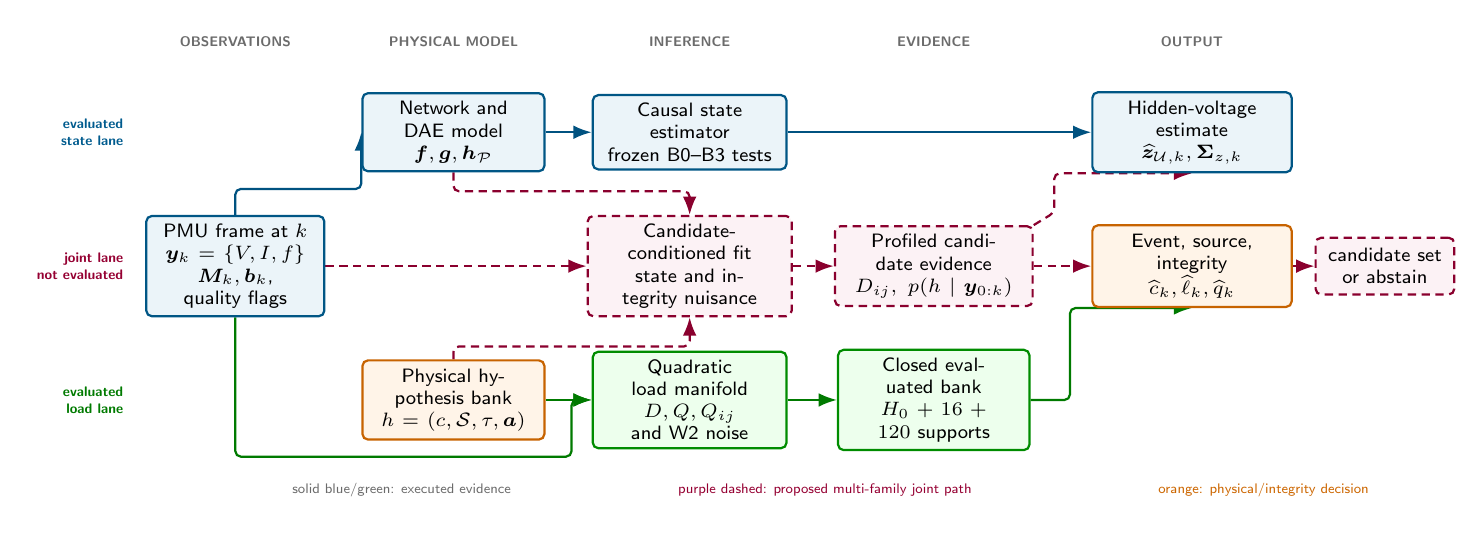
\begin{tikzpicture}[
  x=1cm,y=1cm,
  font=\sffamily\scriptsize,
  >=Latex,
  box/.style={draw=black!55,rounded corners=2pt,thick,align=center,
    minimum height=0.72cm,inner sep=3pt,fill=white},
  state/.style={box,draw=accessblue!75!black,fill=accessblue!8},
  event/.style={box,draw=orange!78!black,fill=orange!9},
  loadcase/.style={box,draw=green!55!black,fill=green!7},
  pending/.style={box,draw=purple!72!black,densely dashed,fill=purple!5},
  arr/.style={->,thick,draw=black!60,rounded corners=2pt},
  pendingarr/.style={->,thick,densely dashed,draw=purple!72!black,rounded corners=2pt},
  lane/.style={font=\sffamily\tiny\bfseries,anchor=east,align=right}
]

% Column headings make the contract readable before the individual boxes.
\foreach \x/\txt in {0.95/OBSERVATIONS,3.72/PHYSICAL MODEL,6.72/INFERENCE,9.82/EVIDENCE,13.10/OUTPUT}{
  \node[font=\sffamily\tiny\bfseries,text=black!58] at (\x,4.35) {\txt};
}

\node[state,text width=2.05cm,minimum height=1.15cm] (pmu) at (0.95,1.50)
  {PMU frame at $k$\\$\bm y_k=\{V,I,f\}$\\$\bm M_k,\bm b_k$, quality flags};

\node[state,text width=2.10cm] (dae) at (3.72,3.20)
  {Network and DAE model\\$\bm f,\bm g,\bm h_{\mathcal P}$};
\node[event,text width=2.10cm] (bank) at (3.72,-0.20)
  {Physical hypothesis bank\\$h=(c,\mathcal S,\tau,\bm a)$};

\node[state,text width=2.25cm] (statefit) at (6.72,3.20)
  {Causal state estimator\\frozen B0--B3 tests};
\node[pending,text width=2.38cm,minimum height=0.90cm] (jointfit) at (6.72,1.50)
  {Candidate-conditioned fit\\state and integrity nuisance};
\node[loadcase,text width=2.25cm] (loadfit) at (6.72,-0.20)
  {Quadratic load manifold\\$D,Q,Q_{ij}$ and W2 noise};

\node[pending,text width=2.30cm,minimum height=0.90cm] (compare) at (9.82,1.50)
  {Profiled candidate evidence\\$D_{ij},\ p(h\mid\bm y_{0:k})$};
\node[loadcase,text width=2.22cm] (loadpost) at (9.82,-0.20)
  {Closed evaluated bank\\$H_0+16+120$ supports};

\node[state,text width=2.32cm] (stateout) at (13.10,3.20)
  {Hidden-voltage estimate\\$\widehat{\bm z}_{\mathcal U,k},\bm\Sigma_{z,k}$};
\node[event,text width=2.32cm] (eventout) at (13.10,1.50)
  {Event, source, integrity\\$\widehat c_k,\widehat\ell_k,\widehat q_k$};
\node[pending,text width=1.55cm] (abstain) at (15.55,1.50)
  {candidate set\\or abstain};

% Three distinct lanes: evaluated state, pending joint inference, and evaluated load-only inference.
\node[lane,text=accessblue!80!black] at (-0.35,3.20) {evaluated\\state lane};
\node[lane,text=purple!78!black] at (-0.35,1.50) {joint lane\\not evaluated};
\node[lane,text=green!48!black] at (-0.35,-0.20) {evaluated\\load lane};

\begin{scope}[on background layer]
  % The observation fan-out uses separate upper, middle, and lower corridors.
  \draw[arr,draw=accessblue!72!black] (pmu.north) -- (0.95,2.48) -| (dae.west);
  \draw[arr,draw=accessblue!72!black] (dae) -- (statefit);
  \draw[arr,draw=accessblue!72!black] (statefit) -- (stateout);

  \draw[pendingarr] (pmu.east) -- (jointfit.west);
  \draw[pendingarr] (dae.south) -- (3.72,2.45) -| (jointfit.north);
  \draw[pendingarr] (bank.north) -- (3.72,0.48) -| (jointfit.south);
  \draw[pendingarr] (jointfit) -- (compare);
  \draw[pendingarr] (compare.east) -- (eventout.west);
  \draw[pendingarr] (compare.north east) -- (11.35,2.18) |- (stateout.south);

  \draw[arr,draw=green!48!black] (pmu.south) -- (0.95,-0.92) -- (5.22,-0.92) |- (loadfit.west);
  \draw[arr,draw=green!48!black] (bank) -- (loadfit);
  \draw[arr,draw=green!48!black] (loadfit) -- (loadpost);
  \draw[arr,draw=green!48!black] (loadpost.east) -- (11.55,-0.20) |- (eventout.south);
  \draw[pendingarr] (eventout) -- (abstain);
\end{scope}

\node[font=\sffamily\tiny,text=black!58,anchor=west] at (1.55,-1.35)
  {solid blue/green: executed evidence};
\node[font=\sffamily\tiny,text=purple!78!black,anchor=west] at (6.45,-1.35)
  {purple dashed: proposed multi-family joint path};
\node[font=\sffamily\tiny,text=orange!80!black,anchor=west] at (12.55,-1.35)
  {orange: physical/integrity decision};
\end{tikzpicture}
}
\caption{Scientific argument and validation boundary. The blue B0--B3 path is an independently evaluated state-reconstruction component. The green path is the implemented batch reference estimator $\mathcal E_{\mathrm B}$. The dashed path is the proposed joint estimator $\mathcal E_{\mathrm J}$; its complete posterior remains unevaluated. The exploratory single-event pilot implements only part of that route.}
\label{fig:joint-architecture}
\end{figure*}

\section{Prior Work and Research Gap}
\label{sec:related-work}

\subsection{State, Algebraic Variable, and Unknown-Input Estimation}

Power-system dynamic state estimation combines machine, control, load, and network models with synchronized measurements; model uncertainty and measurement availability remain persistent constraints \cite{zhao2019dse}. Robust filters address non-Gaussian measurement errors \cite{zhao2018gmukf,li2023eventtriggered}, whereas joint input/state estimators recover exogenous inputs in linear systems \cite{gillijns2007input}, nonlinear DAEs \cite{nugroho2022dae,katanic2024recursive}, and event-triggered or distributed power networks \cite{qu2023joint,nguyen2021unknown}. These estimators do not define a multi-family physical-source bank with a simultaneous integrity state.

Learning methods reconstruct states from sparse measurements by encoding graph structure or power-flow relations. Examples combine graph learning with physics-based estimates \cite{ngo2024pignn}, outlier-resistant estimation and outage identification \cite{yue2024graph}, or topology-aware reconstruction under PMU failures and bad data \cite{moshtagh2025topology}. Robust reconstruction does not, by itself, identify the physical source.

\subsection{Sparse-PMU Event and Source Inference}

PMU event identification uses subspaces, engineered features, transfer learning, and graph models \cite{li2018subspace,yuan2021learning,li2022transfer,yuan2023gnn}. Label-light field-stream detection and scarce-label transfer target event presence or family \cite{cheng2022bigan,abdelhai2021transfer}; physical-source recovery is distinct. Prior localization spans joint classification/localization \cite{pandey2020realtime}, sparse-PMU fault, generation-loss, and outage methods \cite{li2019cnn,azizi2021log,azizi2023line,yildiz2024few}, group-sparse physical dictionaries \cite{wang2024group}, and topology-constrained graph losses \cite{li2024knowledge}.

Model-based outage inference provides the closest classical comparison. Phasor angles support line-outage detection \cite{tate2008outage}; uncertain pre-event state can be marginalized jointly with outage identity and sensor placement \cite{zhao2014outages}; and sequential likelihoods handle stochastic operating variation \cite{chen2016quickest,rovatsos2017outage}. Matched-subspace detectors profile linear nuisance through a generalized likelihood ratio \cite{scharf1994matched}. These are the likelihood and nuisance-elimination precedents used here. Our batch load contract instead uses a sparse voltage/current response dictionary and known onset; it is not a quickest-detection comparison. For the separate causal component, we implement the persistent single-outage recursion of Chen \emph{et al.} with its partial-observation covariance marginalization. Its persistent-line scope determines the eligible comparison; load classification and restoration are not attributed to that algorithm.

Open-set recognition differs from source holdout. Siamese boundaries and generative evidence reject events outside learned classes \cite{kummerow2022siamese,kummerow2023sigmoid,hu2026openset}. Source generalization instead ranks a physically enumerable but unlabeled asset as a counterfactual source.

The pmuBAGE collection supports standardized analytics but does not certify source holdout \cite{foggo2024pmubage}. Integrity is a separate variable: robust recovery distinguishes excursions from outliers \cite{chatterjee2020robust}, while utility examples include missing, locked, quantized, and timing-affected synchrophasors \cite{biswas2025quality}.

The unresolved issue is the evaluation contract. New replicas from trained assets measure interpolation, not source generalization; nuisance variation can also alter conclusions \cite{kummerow2023nuisance}. Reconstruction followed by localization is prior art \cite{zhai2025partial,rimkus2025gnn}, but not under the combined held-source, diagnosability, integrity, and mismatch tests used here.

Frequency and rate-of-change-of-frequency (ROCOF) channels are themselves the output of a dynamic estimation problem rather than ideal derivatives of a noiseless phasor angle. A prior benchmark by the authors compared 16 dynamic frequency estimators spanning six practical groups over 34 disturbance scenarios across ten families, including ramps, phase jumps, harmonics, ringdown, and composite inverter-based-resource event sequences, and found substantial disturbance-dependent latency--robustness trade-offs \cite{Mayorga2026FrequencyBenchmark}. That result motivates treating reported frequency and ROCOF as measured quantities with their own estimator- and disturbance-dependent error, not as an additional noiseless PMU channel.

\subsection{Observability, Diagnosability, and Sensor Value}

Functional observability asks whether a requested function of state can be inferred without full-state observability \cite{fernando2010functional,zhang2025functional}; nonlinear extensions require the observation fibers to determine the requested functional locally, not merely a favorable Jacobian at one point \cite{montanari2022functional}. Unknown-input observability instead asks whether exogenous inputs can be reconstructed from output histories \cite{hou1998input}; fault detectability asks whether a fault can be separated while disturbances are decoupled \cite{nyberg2002detectability}. Sparse strong observability extends the question to corrupted sensor sets \cite{showkatbakhsh2020secure,sun2026secure}, and attack identification characterizes when adversarial input supports are distinguishable from system behavior \cite{pasqualetti2013attack}. Eriksson \emph{et al.} quantify pairwise diagnosability for stochastic linear descriptor models \cite{eriksson2013diagnosability}. Likelihood inference with singular first-order information also has established nonregular asymptotics \cite{rotnitzky2000singular}; therefore, a vanishing projected tangent is not by itself a universal impossibility result. PMU placement based on empirical observability Gramians treats sensor value as task dependent \cite{qi2015placement,sun2016observability}. For event sources, Jamei \emph{et al.} derive placement-dependent fault-localization limits \cite{jamei2020limits}; Conte \emph{et al.} partition a radial grid into indistinguishable line clusters \cite{conte2023fault}; and Yildiz and Abur optimize sparse placement for event detection and identification \cite{yildiz2025sparse}. These results distinguish hidden-state reconstruction, input reconstruction, and pairwise source separation. They also rule out a general optimal-placement claim from one prescribed eight-PMU set.

\begin{table*}[t]
\caption{Research gap by methodological family. The full paper-by-paper capability matrix is reported in Supplementary Appendix~A.}
\label{tab:literature-capability}
\centering
\footnotesize
\begin{tabularx}{\textwidth}{@{}lXXX@{}}
\toprule
Family & Established capability & Remaining issue for this problem & Role here \\
\midrule
Dynamic state and unknown-input estimation \cite{gillijns2007input,nugroho2022dae,katanic2024recursive} & Reconstructs states or unknown inputs from model and PMU histories & Does not usually define a closed physical event-source bank with compositional integrity & Defines the state-reconstruction path and its nuisance variables \\
Learned event localization \cite{pandey2020realtime,li2024knowledge,yildiz2024few} & Detects and localizes represented event families under sparse sensing & Source-label training can confound asset memorization with source generalization & Supplies the supervised baseline and held-source stress test \\
Model-based event inference \cite{tate2008outage,zhao2014outages,chen2016quickest} & Ranks physical outage hypotheses and can marginalize operating uncertainty & Published contracts are event-specific and do not establish the present simultaneous-load problem & Motivates physical candidate likelihoods and nuisance profiling \\
Observability and placement \cite{montanari2022functional,jamei2020limits,yildiz2025sparse} & Characterizes state recovery or event separation for a declared sensing task & Rank alone does not quantify finite-horizon support ambiguity & Supplies the target-recovery and diagnosability tests \\
This work & Reconstructs a requested hidden-voltage field and ranks all load supports with $K\le2$ & The multi-family state/event/integrity posterior remains untested & Connects separate evaluated paths through one information-based formulation \\
\bottomrule
\end{tabularx}
\end{table*}

\subsection{Remaining Technical Gap}

Table~\ref{tab:literature-capability} shows why one accuracy value cannot close the gap. The state path must specify the requested function, and the event path must expose indistinguishable sources before any classifier is trusted. A source-generalization test must also remove the physical asset from every source-labeled fitting step. Under that contract, learning is useful only if it corrects model discrepancy or reduces candidate-search cost without memorizing asset identity.

The experiments cover only part of this intersection. PowerDynamics supports hidden-voltage estimation, physical recentering, and prospective load-source inference. ANDES documents what a supervised representation loses under source holdout. A common multi-family experiment with state and integrity nuisance remains future work.

\section{State, Event, and Source Problem}
\label{sec:problem-formulation}

\subsection{One Physical Model, Two Inference Questions}

Let $\bm x(t)$ and $\bm z(t)$ denote differential and algebraic states, $\bm q(t)$ the network mode, and $\bm\theta$ the operating parameters. A physical candidate is
\begin{equation}
 h=(c,\mathcal S,\tau,\bm a,\bm d),
 \label{eq:physical-hypothesis}
\end{equation}
where $c$ is the event family, $\mathcal S$ its bus or branch support, $\tau$ the onset, $\bm a$ the signed severity, and $\bm d$ the temporal profile. The hybrid plant and measurement boundary are
\begin{align}
 \dot{\bm x}&=\bm f_h(\bm x,\bm z,\bm u;\bm\theta)+\bm w_x, &
 \bm0&=\bm g_h(\bm x,\bm z,\bm u;\bm\theta), \label{eq:dae-model}\\
 \bm y_k&=\bm M_k[\bm h_{\mathcal P_k}(\bm x_k,\bm z_k,\bm q_k;\bm\theta)+\bm b_k]+\bm v_k. \label{eq:dae-measurement}
\end{align}
The event enters the physical equations through $h$. In contrast, $\bm M_k$ records channel availability and $\bm b_k$ records measurement corruption. A physical event and a failed PMU can therefore coexist without becoming a new event class.

For a scheduled impulse-free intervention, the physical switch preserves the
differential state and re-equilibrates the algebraic state in the post-event mode:
\begin{equation}
 \bm x(\tau^+)=\bm x(\tau^-),\qquad
 \bm g_{h^+}\!\left(\bm x(\tau^-),\bm z(\tau^+),\bm u;\bm\theta^+\right)=\bm0.
 \label{eq:event-right-limit}
\end{equation}
This right limit is not necessarily the array stored inside a simulator callback.
The frozen trajectories begin at the first retained 30-Hz frame, so they validate
the sampled response rather than the callback microstate. Supplementary
Appendix~D proves the local consistency expansion and separates the direct
algebraic PMU signature from its subsequent dynamic propagation.

The primary estimated electrical target is the rectangular complex-voltage field,
not a collection of independently learned PMU channels. Conditional on a
physical candidate and its network mode, bus injections, oriented terminal
currents, and complex powers are deterministic functionals of the estimated DAE
state. The network map uses $\bm I=\bm Y_{\mathrm{bus}}\bm V$ and
$S_i=V_iI_i^*$; terminal currents retain the complete branch primitive rather
than replacing it by a bus-injection current. Thus a fault changes a shunt, a
line outage changes $\bm Y_{\mathrm{bus}}$, and generation or load events change
the corresponding injections.

Supplementary Appendix~B defines the corresponding electrical output maps and
their frequency, ROCOF, and balanced-waveform qualifications. They belong to
the proposed joint estimator $\mathcal E_{\mathrm J}$; the implemented batch
event estimator $\mathcal E_{\mathrm B}$ does not infer a state trajectory or
virtual outputs. Only hidden complex voltage is empirically validated by the
separate state-reconstruction component.

The first question asks for a function of state. With PMUs at
\begin{equation}
 \mathcal P=\{2,5,6,10,19,22,29,39\},
 \label{eq:pmu-set}
\end{equation}
the requested target is the complex voltage at the remaining 31 buses. The state estimator uses rectangular voltage and controlled terminal-current channels. The second question asks which physical candidate generated the observed response. For the evaluated load family,
\begin{equation}
 \mathcal S\subseteq\mathcal L,\qquad |\mathcal L|=16,\qquad
 K=|\mathcal S|\le2,
 \label{eq:sparse-load-support}
\end{equation}
which yields one no-event hypothesis, 16 single-source hypotheses, and 120 two-source supports.

\begin{figure*}[t]
\centering
\resizebox{\textwidth}{!}{% Vector reconstruction of the IEEE 39-bus network used in the manuscript.
% Branches and PMU locations were checked against the frozen topology manifest;
% coordinates are schematic and never enter an electrical-distance calculation.
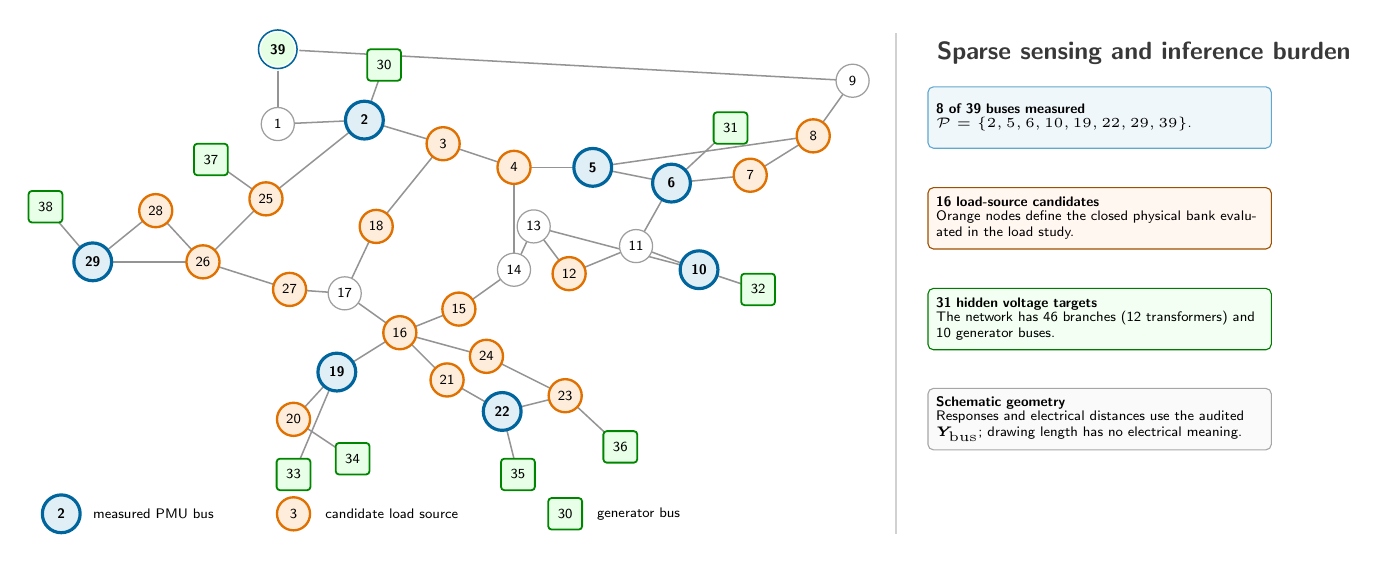
\begin{tikzpicture}[
  x=1cm,y=1cm,
  font=\sffamily\scriptsize,
  bus/.style={circle,draw=black!38,fill=white,line width=0.45pt,
    minimum size=0.42cm,inner sep=0.25pt,font=\sffamily\tiny},
  source/.style={bus,draw=orange!88!black,fill=orange!14,line width=0.85pt},
  pmu/.style={bus,draw=accessblue!88!black,fill=accessblue!12,
    line width=1.15pt,minimum size=0.48cm,font=\sffamily\tiny\bfseries},
  gen/.style={rounded corners=1.2pt,draw=green!52!black,fill=green!9,
    line width=0.65pt,minimum width=0.43cm,minimum height=0.40cm,
    inner sep=0.25pt,font=\sffamily\tiny},
  pmugen/.style={circle,double=accessblue!88!black,double distance=0.55pt,
    draw=white,fill=green!10,line width=0.55pt,minimum size=0.49cm,
    inner sep=0.25pt,font=\sffamily\tiny\bfseries},
  branch/.style={draw=black!42,line width=0.55pt,line cap=round},
  note/.style={rounded corners=2pt,align=left,text width=4.15cm,
    minimum height=0.78cm,inner sep=3pt,font=\sffamily\tiny},
  rule/.style={draw=black!18,line width=0.45pt}
]

% Network geometry adapted from the project slide deck and redrawn as vector art.
\coordinate (b1c) at (0.0,2.1);
\coordinate (b2c) at (1.1,2.15);
\coordinate (b3c) at (2.1,1.85);
\coordinate (b4c) at (3.0,1.55);
\coordinate (b5c) at (4.0,1.55);
\coordinate (b6c) at (5.0,1.35);
\coordinate (b7c) at (6.0,1.45);
\coordinate (b8c) at (6.8,1.95);
\coordinate (b9c) at (7.3,2.65);
\coordinate (b39c) at (0.0,3.05);
\coordinate (b10c) at (5.35,0.25);
\coordinate (b11c) at (4.55,0.55);
\coordinate (b12c) at (3.70,0.20);
\coordinate (b13c) at (3.25,0.80);
\coordinate (b14c) at (3.00,0.25);
\coordinate (b15c) at (2.30,-0.25);
\coordinate (b16c) at (1.55,-0.55);
\coordinate (b17c) at (0.85,-0.05);
\coordinate (b18c) at (1.25,0.80);
\coordinate (b19c) at (0.75,-1.05);
\coordinate (b20c) at (0.2,-1.65);
\coordinate (b21c) at (2.15,-1.15);
\coordinate (b22c) at (2.85,-1.55);
\coordinate (b23c) at (3.65,-1.35);
\coordinate (b24c) at (2.65,-0.85);
\coordinate (b25c) at (-0.15,1.15);
\coordinate (b26c) at (-0.95,0.35);
\coordinate (b27c) at (0.15,0.00);
\coordinate (b28c) at (-1.55,1.00);
\coordinate (b29c) at (-2.35,0.35);
\coordinate (b30c) at (1.35,2.85);
\coordinate (b31c) at (5.75,2.05);
\coordinate (b32c) at (6.10,0.00);
\coordinate (b33c) at (0.20,-2.35);
\coordinate (b34c) at (0.95,-2.15);
\coordinate (b35c) at (3.05,-2.35);
\coordinate (b36c) at (4.35,-2.00);
\coordinate (b37c) at (-0.85,1.65);
\coordinate (b38c) at (-2.95,1.05);

% The 46 physical branches are drawn before the buses so labels remain legible.
\foreach \a/\b in {
  1/2,1/39,2/3,2/25,2/30,3/4,3/18,4/5,4/14,5/6,5/8,
  6/7,6/11,6/31,7/8,8/9,9/39,10/11,10/13,10/32,11/12,
  12/13,13/14,14/15,15/16,16/17,16/19,16/21,16/24,17/18,
  17/27,19/20,19/33,20/34,21/22,22/23,22/35,23/24,23/36,
  25/26,25/37,26/27,26/28,26/29,28/29,29/38}{
    \draw[branch] (b\a c) -- (b\b c);
}

% Uninstrumented, noncandidate transmission buses.
\foreach \n in {1,9,11,13,14,17}{\node[bus] (b\n) at (b\n c) {\n};}

% Candidate load-source buses in the evaluated physical dictionary.
\foreach \n in {3,4,7,8,12,15,16,18,20,21,23,24,25,26,27,28}{
  \node[source] (b\n) at (b\n c) {\n};
}

% Prescribed PMU buses. Bus 39 is both a PMU and a generator bus.
\foreach \n in {2,5,6,10,19,22,29}{\node[pmu] (b\n) at (b\n c) {\n};}
\node[pmugen] (b39) at (b39c) {39};

% Remaining generator buses.
\foreach \n in {30,31,32,33,34,35,36,37,38}{\node[gen] (b\n) at (b\n c) {\n};}

% Small legend under the topology.
\node[pmu] (lpmu) at (-2.75,-2.85) {2};
\node[anchor=west,font=\sffamily\tiny] at (-2.47,-2.85) {measured PMU bus};
\node[source] (lsrc) at (0.20,-2.85) {3};
\node[anchor=west,font=\sffamily\tiny] at (0.48,-2.85) {candidate load source};
\node[gen] (lgen) at (3.65,-2.85) {30};
\node[anchor=west,font=\sffamily\tiny] at (3.93,-2.85) {generator bus};

% Right-hand reading guide turns the topology into part of the scientific argument.
\draw[rule] (7.85,-3.10) -- (7.85,3.25);
\node[anchor=west,font=\sffamily\small\bfseries,text=black!78] at (8.25,3.00)
  {Sparse sensing and inference burden};

\node[note,anchor=north west,draw=accessblue!62,fill=accessblue!6]
  at (8.25,2.58) {\textbf{8 of 39 buses measured}\\[-1pt]
  $\mathcal P=\{2,5,6,10,19,22,29,39\}$.};

\node[note,anchor=north west,draw=orange!62!black,fill=orange!6]
  at (8.25,1.30) {\textbf{16 load-source candidates}\\[-1pt]
  Orange nodes define the closed physical bank evaluated in the load study.};

\node[note,anchor=north west,draw=green!48!black,fill=green!5]
  at (8.25,0.02) {\textbf{31 hidden voltage targets}\\[-1pt]
  The network has 46 branches (12 transformers) and 10 generator buses.};

\node[note,anchor=north west,draw=black!35,fill=black!2]
  at (8.25,-1.25) {\textbf{Schematic geometry}\\[-1pt]
  Responses and electrical distances use the audited $\bm Y_{\rm bus}$; drawing length has no electrical meaning.};
\end{tikzpicture}
}
\caption{Sensing and candidate geometry on the IEEE 39-bus system. Blue circles mark the eight PMU buses, orange circles the 16 evaluated load-source buses, and green boxes generator buses. The drawing preserves the audited 46-branch connectivity but does not encode geographic or electrical distance.}
\label{fig:ieee39-topology}
\end{figure*}

\subsection{Physical Events and Measurement Integrity}

The historical event bank has eight abnormal labels, but the label number is not the scientific variable. Table~\ref{tab:event-ontology} rewrites the bank as four physical interventions, two integrity states, and two prescribed compositions. This representation matters because a missing packet identifies an integrity source directly while reducing the information available for physical-source inference.

\begin{table*}[t]
\caption{Event ontology and historical ANDES inventory. Each source configuration has five replicas. Physical and integrity sources remain separate outputs.}
\label{tab:event-ontology}
\centering
\footnotesize
\begin{tabularx}{\textwidth}{@{}cXlllr@{}}
\toprule
ID & Operational meaning & Physical intervention & Physical source & Integrity state/source & Records \\
\midrule
0 & Normal operation & none & none & nominal & 5 \\
1 & Bus fault & fault admittance & bus & nominal & 195 \\
2 & Line outage & topology removal & branch & nominal & 170 \\
3 & Generation change & active/reactive injection & generator bus & nominal & 50 \\
4 & Load change & active/reactive withdrawal & load bus & nominal & 90 \\
5 & Missing data & none & none & dropout / PMU & 40 \\
6 & Generation change with missing data & generation change & generator bus & dropout / PMU & 50 \\
7 & Bad data & none & none & corruption / PMU channel & 40 \\
8 & Prescribed mixed disturbance & generation plus load changes & declared generator bus & measurement disturbance / PMU & 50 \\
\midrule
 & Total & & & & 690 \\
\bottomrule
\end{tabularx}
\end{table*}

The desired decision consists of the hidden-voltage estimate, its uncertainty, the physical family and support, and the integrity state. These components use different correctness tests. Hidden-voltage relative error is averaged over a complete trajectory and the 31 requested buses. Event detection, family classification, exact-support recovery, and integrity localization retain their own populations. A joint decision is correct only when every applicable component is correct.

Causality and generalization are also explicit. A causal estimate at time $k$ may use only $\bm y_{0:k}$; fixed-lag or complete-window results are retrospective. A held-source test removes the physical asset from every source-labeled fitting and tuning step. Confidence intervals use trajectories, event parents, or rebuilt plants as independent units, never individual 30-Hz samples. Supplementary Appendix~C records the exact metrics and event operators.

\section{What Sparse Measurements Can Determine}
\label{sec:functional-observability}

The analysis separates two questions before an estimator is chosen. The first asks whether the measured history determines the requested hidden-voltage function. The second asks whether it distinguishes competing event supports. Both depend on the sensing geometry, but they fail for different reasons.

\subsection{Recovering a Requested Voltage Function}

Linearizing the index-reduced DAE around a verified equilibrium gives
\begin{align}
 \delta\bm x_{k+1}&=\bm A_d\delta\bm x_k+\bm w_k,&
 \delta\bm y_k&=\bm C\delta\bm x_k+\bm v_k,\label{eq:local-model}\\
 \delta\bm z_{\mathcal U,k}&=\bm L_{\mathcal U}\delta\bm x_k. \nonumber
\end{align}
Here $\delta\bm x_k\in\mathbb R^{114}$, the 32 measured channels form $\delta\bm y_k$, and the 62 rectangular voltage components at the 31 unmeasured buses form the target. For a horizon of $N$ transitions, let
\begin{equation}
 \mathcal O_N=\operatorname{col}(\bm C,\bm C\bm A_d,\ldots,\bm C\bm A_d^N),
 \qquad \bm L_r=\bm L_{\mathcal U}\bm A_d^r.
 \label{eq:observability-matrix}
\end{equation}

\begin{proposition}[Finite-horizon functional reconstruction]
\label{prop:functional-reconstruction}
The noise-free measurement history through $N$ uniquely determines the requested voltage at time $r\le N$ if and only if
\begin{equation}
 \ker\mathcal O_N\subseteq\ker\bm L_r.
 \label{eq:functional-condition}
\end{equation}
\end{proposition}

The condition is weaker than full-state observability: unobservable state directions are harmless when they do not change the requested voltage. Under Gaussian noise, the same row-space condition yields the minimum-variance linear unbiased target estimate; its covariance depends on singular values and target alignment, not rank alone \cite{fernando2010functional,zhang2025functional}. Supplementary Appendix~D gives the proof, the covariance expression, and the nonlinear constant-rank qualification \cite{montanari2022functional}.

The numerical audit illustrates why that qualification matters. The original implementation formed $\mathcal O_N^{\mathsf T}\mathcal O_N$ and applied a relative eigenvalue threshold. Its pseudo-rank rises and then falls as samples are added, which an exact observability rank cannot do. Figure~\ref{fig:observability-horizon} therefore separates two conclusions. Longer history improves numerical conditioning, but the tested computation does not certify full-state or exact functional observability. The nonlinear estimator is evaluated independently.

\begin{figure*}[t]
\centering
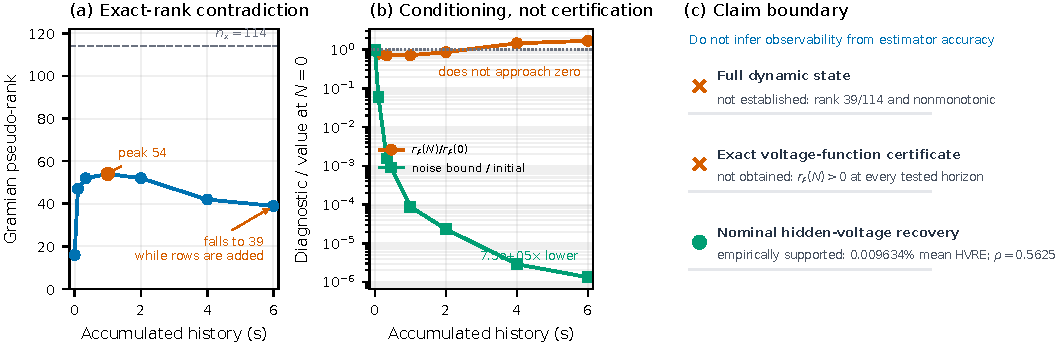
\includegraphics[width=\textwidth]{figures/generated/observability_horizon.pdf}
\caption{Structural audit and claim boundary. Adding history lowers the target-noise bound, but the relative-threshold pseudo-rank is nonmonotone and the target residual remains nonzero. The audit therefore motivates a conditioning analysis; it does not prove full-state or exact hidden-voltage observability.}
\label{fig:observability-horizon}
\end{figure*}

The bus-level residual from this audit was frozen before the nonlinear TEST trajectories were scored. Its association with empirical bus error is used only as an exploratory theory-to-data check because the projector remains threshold sensitive. An SVD-based, noise-tied rank audit is still required for a structural certificate.

\subsection{Distinguishing Event Supports}

Source inference introduces a different nuisance space. Under candidate $h$, stack the available measurements over $H$ samples as
\begin{equation}
 \bm Y_H=\bm s_{h,H}+\mathcal O_{h,H}\bm\xi_h
 +\mathcal E_{S,H}\bm\beta_h+\bm\varepsilon_H,
 \label{eq:stacked-hypothesis}
\end{equation}
where $\bm s_{h,H}$ is the physical response, $\bm\xi_h$ an admissible initial-state deviation, and $\mathcal E_{S,H}\bm\beta_h$ corruption on integrity support $S$. Each candidate therefore defines an affine response manifold. For candidates $i$ and $j$, their profiled separation is
\begin{equation}
 \begin{aligned}
 D_{ij,S}(H)=\frac12\min_{\bm\xi_i,\bm\xi_j,\bm\beta}
 \bigl\|{}&\bm s_{i,H}+\mathcal O_{i,H}\bm\xi_i\\[-1mm]
 &-\bm s_{j,H}-\mathcal O_{j,H}\bm\xi_j
 +\mathcal E_{S,H}\bm\beta\bigr\|_{\bm R_H^{-1}}^2.
 \end{aligned}
 \label{eq:pairwise-information}
\end{equation}
This distance profiles the nuisance directions that either candidate can use to explain the same measurements. It specializes descriptor-model diagnosability and matched-subspace testing to the PMU event bank \cite{eriksson2013diagnosability,scharf1994matched}.

\begin{proposition}[Local candidate indistinguishability]
\label{prop:source-indistinguishability}
If $D_{ij,S}(H)=0$, the two candidate manifolds intersect. At an intersection they induce the same Gaussian measurement law, so no rule can distinguish them uniformly over the declared nuisance set.
\end{proposition}

A positive distance establishes local separation, not an easy decision. Small distance or near-collinear signatures amplify noise and delay support resolution. Supplementary Appendix~D proves the proposition, treats unknown sparse corruption, and shows that adding a conditionally independent PMU cannot reduce the profiled margin when the nuisance contract is fixed.

The infinitesimal version makes the first-order boundary explicit. Let
$\bm g_\star$ be the event-response tangent, $\bm J_c$ the tangent of the closest
competing nuisance manifold, and $\bm W^{\mathsf T}\bm W=\bm R_H^{-1}$. With
\begin{equation}
 \gamma_1^2=\|\left(\bm I-\bm P_c\right)\bm W\bm g_\star\|_2^2,
 \qquad
 \bm P_c=(\bm W\bm J_c)(\bm W\bm J_c)^{\dagger},
 \label{eq:profiled-first-order-coefficient}
\end{equation}
the corresponding local version of \eqref{eq:pairwise-information} satisfies
$D_{\star c}(a)=a^2\gamma_1^2/2+o(a^2)$. Thus $\gamma_1>0$ gives
first-order separation after nuisance fitting; $\gamma_1=0$ only makes the
first-order test inconclusive. Relative curvature can then produce an $a^4$
squared-distance law. The full statement and proof are in Supplementary
Appendix~D. The present experiments do not yet test the convergence of
$2D_{\star c}(a)/a^2$ to $\gamma_1^2$.

For multiple events, let $\bm G$ collect the first-order event signatures,
$\bm N$ the nuisance tangent, let $\bm P_{\bm A}$ denote the orthogonal
projector onto $\operatorname{range}(\bm A)$, and define
$\overline{\bm G}=(\bm I-\bm P_{\bm W\bm N})\bm W\bm G$ the event dictionary
after nuisance removal. All first-order event information that survives
worst-case nuisance fitting lies in
$\mathcal D=\operatorname{range}(\overline{\bm G})$. Hence
$d_{\mathcal D}=\operatorname{rank}(\overline{\bm G})$ is the intrinsic linear
diagnostic dimension, not the number of retained PMU channels or reconstructed
states. Supplementary Appendix~D proves that coordinates on $\mathcal D$
preserve every profiled Gaussian likelihood ratio when candidates share the
same nuisance range. For true support $S$, severity direction
$\bm\alpha_S$, and competing support $C$, the support-to-support margin is
\begin{equation}
 \gamma_{S\rightarrow C}^2(\bm\alpha_S)
 =\|\left(\bm I-\bm P_{\overline{\bm G}_C}\right)
 \overline{\bm G}_S\bm\alpha_S\|_2^2.
 \label{eq:support-to-support-margin}
\end{equation}
Equation~\eqref{eq:support-to-support-margin} is exact for signed amplitudes or
an interior parameter point. At a physical boundary, let
$T_{\mathcal A_C}(\bm0)$ be the tangent cone of the competitor's admissible
amplitude domain. The first-order physical margin is instead
\begin{equation}
 \gamma_{\mathrm{phys}}^2
 =\min_{\bm u,\,\bm\beta_C\in T_{\mathcal A_C}(\bm0)}
 \|\bm W\bm G_S\bm\alpha_S-\bm W\bm N\bm u
       -\bm W\bm G_C\bm\beta_C\|_2^2.
 \label{eq:physical-cone-margin}
\end{equation}
Because the cone is contained in its span,
$\gamma_{\mathrm{phys}}\ge\gamma_{S\rightarrow C}$; zero relaxed margin does
not prove ambiguity for a one-sided event. Shared sources cancel exactly only
when the matched amplitude is feasible and the relevant constraint is inactive.
Competitor enrichment still cannot increase the margin, and a nested superset
still has zero margin when its added amplitude admits zero. Geometry can
therefore rank non-nested explanations, but cardinality among nested supports
requires a model-selection penalty or integrated evidence. Supplementary
Appendix~D proves the subspace and cone statements.

For persistent load events, subtract the common no-event trajectory and write the $T$-sample response as
\begin{equation}
 \bm Y_T=\mathcal H_T\bm a+\bm\varepsilon_T.
 \label{eq:persistent-event-model}
\end{equation}
Let $\mathcal A_{2K}$ contain vectors with at most $2K$ nonzero entries.

\begin{proposition}[Finite-horizon sparse event injectivity]
\label{prop:sparse-event-injectivity}
Every event with at most $K$ active sources is uniquely determined in the noise-free model if and only if
\begin{equation}
 \ker\mathcal H_T\cap\mathcal A_{2K}=\{\bm0\}.
 \label{eq:sparse-injectivity-condition}
\end{equation}
Stable amplitude estimation also requires a well-conditioned support Gramian.
\end{proposition}

The proposition distinguishes uniqueness from finite-information difficulty. With prefix-consistent causal whitening, adding samples cannot reduce the profiled separation between two fixed supports. Separation grows when their steady signatures differ and can saturate when only a finite transient distinguishes them. The experiments therefore ask two questions in order: does the posterior identify how many sources are active, and does the remaining separation identify which sources? Full proofs and the temporal cases appear in Supplementary Appendix~D.

The separation also has an operational meaning under the corresponding simple
equal-covariance Gaussian quotient experiment. If $d$ is the nuisance-profiled
Mahalanobis distance, then
\begin{equation}
 P_e^\star=\Phi(-d/2),\qquad
 D_{\mathrm{KL}}=d^2/2.
 \label{eq:gaussian-operational-separation}
\end{equation}
Thus a local order-$k$ pair satisfying
$d_T^2(a)=T\mathcal I_k|a|^{2k}+o(T|a|^{2k})$, with
$\mathcal I_k>0$, has the resolution scale
\begin{equation}
 |a|_{\min}(\alpha,T)\sim
 \left[\frac{2\Phi^{-1}(1-\alpha)}{\sqrt{T\mathcal I_k}}
 \right]^{1/k}.
 \label{eq:order-k-resolution-scale}
\end{equation}
First-order and curvature-only separation therefore improve as $T^{-1/2}$ and
$T^{-1/4}$, respectively. Equation~\eqref{eq:gaussian-operational-separation}
is exact for the stated quotient experiment, not for an amplitude-marginalized
nonlinear support mixture.

Two limits prevent accuracy from being interpreted without a severity and
candidate-set contract. If an added active amplitude may approach zero, its law
approaches the nested lower-cardinality law, so uniform exact-support recovery
is impossible without a minimum-severity condition or abstention. For $M$
equiprobable supports, Fano's inequality further gives
\begin{equation}
 \begin{aligned}
 P_e&\geq\left[1-\frac{\overline D_{\mathrm{KL}}+\log 2}{\log M}
 \right]_+,\\
 \overline D_{\mathrm{KL}}&=\frac{1}{M^2}
 \sum_{i,j}D_{\mathrm{KL}}(P_i\Vert P_j).
 \end{aligned}
 \label{eq:fano-support-bound}
\end{equation}
which separates algorithmic failure from insufficient physical information
\cite{cover2006elements,tsybakov2009nonparametric}. Supplementary Appendix~D
states the assumptions, proofs, and the resulting necessary horizon bound.

\section{Evaluated Components and Two Estimator Contracts}
\label{sec:estimation}

Figure~\ref{fig:joint-architecture} separates three objects that must not share
one name. The blue B0--B3 state reconstructor is an independently evaluated
component. The green path is the implemented reference event estimator,
$\mathcal E_{\mathrm B}$, a batch physical-manifold Bayesian bank. The dashed
path is the second estimator proposal, $\mathcal E_{\mathrm J}$, a joint
Hybrid-DAE state--event Bayesian model that remains unexecuted. They share the
plant and PMU operator, but no fitted posterior is shared in the present results.

\subsection{Causal State Reconstruction}

The state experiment changes one information source at a time. It validates a
state-reconstruction component, not the joint estimator $\mathcal E_{\mathrm J}$.
B0 returns the equilibrium voltage. B1 conditions that equilibrium on the current PMU frame. B2 propagates the state causally and then applies the PMU correction. B3 is a retrospective fixed-lag smoother used only to test whether later measurements add useful information. This sequence isolates where each improvement comes from.

For the local model in \eqref{eq:local-model}, B2 uses the standard Kalman recursion \cite{kalman1960}:
\begin{align}
 \widehat{\bm x}_{k|k-1}&=\bm A_d\widehat{\bm x}_{k-1|k-1},
 \nonumber\\[-1mm]
 \bm P_{k|k-1}&=\bm A_d\bm P_{k-1|k-1}\bm A_d^{\mathsf T}+\bm Q,
 \nonumber\\
 \bm K_k&=\bm P_{k|k-1}\bm C^{\mathsf T}
 (\bm C\bm P_{k|k-1}\bm C^{\mathsf T}+\bm R)^{-1},
 \nonumber\\
 \widehat{\bm x}_{k|k}&=\widehat{\bm x}_{k|k-1}
 +\bm K_k\bm\nu_k. \label{eq:kf-compact}
\end{align}
The hidden-voltage estimate is $\bm z_{\mathcal U,0}+\bm L_{\mathcal U}\widehat{\bm x}_{k|k}$. Only measurements through $k$ enter B2. B3 follows the Gaussian backward recursion \cite{rauch1965smoothing} and is explicitly retrospective.

Two checks separate point accuracy from uncertainty. First, a temperature map fitted on independent calibration trajectories rescales the two rectangular voltage components without changing the state estimate. Second, an observed-innovation statistic tests whether the nominal model has become inadequate. Neither operation repairs the physical model. Their complete equations and negative discrepancy ablations appear in Supplementary Appendix~E.

When the operating point is stale, the physical-recentering estimator rebuilds a feasible equilibrium instead of shifting measured voltages by an unconstrained offset. It solves
\begin{equation}
 \begin{aligned}
 (\widehat{\bm V},\widehat{\bm d})
 =\arg\min_{\bm V,\bm d}\; &\|\bm e_y(\bm V)\|_2^2
 +\gamma^2\|\bm g_{\mathrm{AC}}(\bm V,\bm d)\|_2^2\\[-1mm]
 &+\lambda q_d^{-2}\|\bm d\|_2^2,
 \end{aligned}
 \label{eq:e06h-map}
\end{equation}
where $\bm e_y$ uses only measured voltage and terminal-current phasors, $\bm g_{\mathrm{AC}}$ enforces AC balance and bus conventions, and $\bm d$ collects admissible load and generation changes. Development data fix the weights and continuation rule before TEST. Hidden voltages and the true nuisance vector never enter the solve.

\subsection{Implemented Batch Physical-Manifold Bayes $\mathcal E_{\mathrm B}$}
\label{sec:load-event-inference}

The reference estimator targets
$p_{\mathrm B}(S,\bm a_S\mid\bm r,\bm\eta_0,\tau_0,c_{\rm load})$:
operating point, onset, and family are fixed, while support and amplitudes are
inferred. The physical question is what the measured PMUs would have recorded
if a candidate load bus had changed. For each of the 16 buses, centered nonlinear simulations form the unit response
\begin{equation}
 \bm D_g=\frac{\bm y_g(+\epsilon)-\bm y_g(-\epsilon)}{2\epsilon},
 \qquad \epsilon=0.005.
 \label{eq:load-tangent}
\end{equation}
Symmetric simulations also estimate source self-curvature $\bm Q_i$ and pairwise interaction $\bm Q_{ij}$. The mean response for support $S$ is
\begin{equation}
 \bm\mu_S(\bm a)=\sum_{i\in S}(a_i\bm D_i+a_i^2\bm Q_i)
 +\sum_{\substack{i,j\in S\\i<j}}a_ia_j\bm Q_{ij}.
 \label{eq:load-multi-source-mean}
\end{equation}
The mixed term matters physically: two simultaneous interventions need not equal the sum of two isolated responses.

After subtracting the normal mean, the residual follows
$\bm r=\bm\mu_S(\bm a)+\bm\varepsilon$ under the frozen Gaussian covariance. Each support receives normalized evidence by integrating over its active amplitudes,
\begin{align}
 Z_S&=\int \mathcal N(\bm r;\bm\mu_S(\bm a),\bm\Sigma)
 \prod_{i\in S}p(a_i)\,d\bm a_S,\nonumber\\
 p(S\mid\bm r)&\propto Z_S\,\frac{p(|S|)}{\binom{16}{|S|}}.
 \label{eq:load-support-posterior}
\end{align}
Gauss--Hermite quadrature evaluates every support; independent Gauss--Kronrod calculations check representative two-dimensional integrals. Priors, covariance estimation, quadrature order, and calibration checks are documented in Supplementary Appendix~E.
Thus $\mathcal E_{\mathrm B}$ marginalizes one- and two-dimensional amplitudes
rather than substituting a MAP amplitude and local Laplace approximation. The
quadrature is accurate for the frozen second-order physical surrogate; it is not
an exact posterior for the full nonlinear DAE.

The amplitude integral is structurally necessary, not decorative. A superset can
reproduce any smaller support by driving its additional amplitudes to zero, so its
pure profiled geometric distance can also be zero. Integrated evidence accounts
for the volume of amplitude values that fit the data, while $p(|S|)$ and the
within-cardinality prior state the sparsity contract. Cardinality is therefore a
Bayesian model-selection question; it cannot be recovered from best-fit distance
alone.

The evaluated load bank uses a proper signed Gaussian amplitude prior because
load changes may increase or decrease. A one-sided fault, trip, or outage instead
requires a proper truncated slab and boundary-aware evidence. In the local
single-amplitude Gaussian model, Supplementary Appendix~E shows that a
half-normal slab multiplies the signed Bayes factor by an exact directional
factor $2\Phi(z)$. This extension is part of the proposed $\mathcal E_{\mathrm J}$ design; it is
not an evaluated multi-family result.

The posterior is read in a fixed order. First, $p(K\mid\bm r)$ asks whether no source, one source, or two sources are active. Conditional support ranks then ask which buses are involved. Amplitude intervals answer how large the changes are. This order is essential under limited observability because cardinality can be well supported while several source pairs remain plausible.

The prospective experiment evaluates all \GlobalHypothesisCount{} supports at a known onset and fixed PMU set. It conditions on the nominal initial state and assumes no corrupted channels. Thus it evaluates the sparse load specialization of Proposition~\ref{prop:sparse-event-injectivity}, not the full state-and-integrity nuisance model in \eqref{eq:stacked-hypothesis}.

\subsection{Proposed Joint Hybrid-DAE Bayes $\mathcal E_{\mathrm J}$}

The second proposal targets a candidate-conditioned joint posterior over state,
operating nuisance, event family, onset, support, amplitude, and integrity, with
normalized evidence across physical hypotheses. A sequential implementation of
$\mathcal E_{\mathrm B}$ is not a third estimator: under the same prefix and
initial AR(1) density, it must reproduce the batch posterior numerically.

More generally, define the restriction $\mathcal R_0$ to fix
$\bm\eta=\bm\eta_0$, $\tau=\tau_0$, and $c=c_{\rm load}$ and to reuse the same
137-support surrogate, covariance, and priors. The mandatory reduction test is
\begin{equation}
 p_{\mathrm J}(S,\bm a_S\mid\bm Y,\mathcal R_0)
 =p_{\mathrm B}(S,\bm a_S\mid\bm r,\bm\eta_0,\tau_0,c_{\rm load}).
 \label{eq:joint-to-batch-reduction}
\end{equation}
Failure of \eqref{eq:joint-to-batch-reduction} is either an implementation error
or an undeclared change of statistical model.

Iterated smoothing,
Gauss--Newton steps, moving-horizon optimization, or generalized EM would be
numerical realizations of that object, not different scientific estimators.
Changing the solver cannot change the declared priors, candidate set, causal
data boundary, or evidence normalization.
Where the active amplitude remains one- or two-dimensional, the design should
retain quadrature marginalization and use optimization or Laplace only for the
remaining state and nuisance coordinates. For each candidate, virtual electrical outputs are deterministic functionals of
the same state trajectory and network mode. Model averaging must therefore
propagate both within-candidate state uncertainty and between-candidate event
ambiguity; it does not require a separate regressor for every output channel.

A learned component could then correct candidate residuals or reduce the search, but it must not consume source identity as a shortcut. It must also preserve the directions that distinguish critical physical candidates. After whitening and nuisance removal, a rank-$q$ discrepancy basis $\bm Q_D$ with variance $\tau^2$ retains the worst-case fraction
\begin{equation}
 \rho=1-\frac{\tau^2}{1+\tau^2}
 \sigma_{\max}^2(\bm Q_U^{\mathsf T}\bm Q_D)
 \label{eq:discrepancy-retention-main}
\end{equation}
of the information in a protected discriminant subspace $\bm Q_U$. Supplementary Appendix~D derives the corresponding finite-variance rule using the full Gaussian likelihood; maximizing residual accommodation alone would omit its log-determinant penalty. The required common-contract ablation remains learned-only, physics-only, physics plus learned discrepancy, and diagnosability-aware inference with abstention. None of those integrations is presented as an executed result here; Supplementary Appendix~E records the full generative objective so the proposed extension is unambiguous.

\subsection{Exploratory Numerical Route to Multi-Family Inference}
\label{sec:single-event-route}

The joint target $\mathcal E_{\mathrm J}$ in the preceding subsection is a statistical specification, not an executed end-to-end result. A separate single-event pilot implements parts of its physical search and continuous state--severity fit. It uses 32 rectangular voltage/current channels from the same eight PMU buses at 30~Hz; frequency and ROCOF from the historical competition files are not inputs to this likelihood. Its candidate catalog contains $H_0$, bus faults, load changes, generator-reference changes, and branch outages. The generator and line scenarios in this pilot have recovery semantics that must be matched by each candidate's temporal operator. Supplementary Appendix~H records the exact contract and the unverified evidence boundary.

For a fixed family, source, and onset, let $\bm X$ collect the differential trajectory after algebraic projection and let $\bm\vartheta_H$ contain the continuous severity coordinates. Set $\bm r^{\rm dyn}_{H,k}=\bm x_{k+1}-\bm F_{H,k}(\bm x_k;\bm\vartheta_H)$ and $\bm r^{\rm pmu}_{H,k}=\bm y_k-\bm h_{H,k}(\bm x_k;\bm\vartheta_H)$. The pilot minimizes the conditional Gaussian MAP objective
\begin{equation}
\begin{aligned}
J_H(\bm X,\bm\vartheta_H)={}&
\tfrac12\|\bm x_0-\overline{\bm x}_0\|_{\bm P_0^{-1}}^2
+\tfrac12\sum_k\|\bm r^{\rm dyn}_{H,k}\|_{\bm Q^{-1}}^2\\
&+\tfrac12\sum_k\|\bm r^{\rm pmu}_{H,k}\|_{\bm R^{-1}}^2
-\log p(\bm\vartheta_H\mid H).
\end{aligned}
\label{eq:pilot-map}
\end{equation}
The DAE transition $\bm F_{H,k}$ changes with the physical operator: a fault adds a temporary shunt, an outage removes a branch primitive, a load event changes withdrawal, and a generator event perturbs a governor reference. Algebraic sensitivity alone is blind to that last pathway; its PMU effect appears after differential propagation. The objective is conditional on the candidate and the declared Gaussian approximation. A minimum of $J_H$ is not a normalized model probability.

The numerical update uses structured Gauss--Newton smoothing, whose relationship to the iterated extended Kalman smoother is established \cite{bell1994ieks,sarkka2020linesearch}. Partition its local normal equations into trajectory and event-parameter blocks. If $\bm H_{XX}$ is nonsingular, eliminating the trajectory step gives
\begin{equation}
\begin{aligned}
\bm S_H&=\bm H_{\vartheta\vartheta}
-\bm H_{\vartheta X}\bm H_{XX}^{-1}\bm H_{X\vartheta},\\
\bm b_H&=\bm g_{\vartheta}
-\bm H_{\vartheta X}\bm H_{XX}^{-1}\bm g_X,\\
\Delta\bm\vartheta_H&=-\bm S_H^{-1}\bm b_H,\quad
\Delta\bm X=-\bm H_{XX}^{-1}
(\bm g_X+\bm H_{X\vartheta}\Delta\bm\vartheta_H).
\end{aligned}
\label{eq:pilot-schur}
\end{equation}
One Armijo factor is applied to both increments and tested against the nonlinear objective. Equation~\eqref{eq:pilot-schur} is algebraically the full joint step; calling $\bm b_H$ a gradient of the \emph{profiled} objective additionally requires the trajectory to be conditionally stationary. The appendix derives both statements and explains the numerical guards.

The pilot separates proposal recall from final selection. An $H_0$ innovation detector identifies an alarm window; the onset is refined separately, and a common pre-event state is fitted without event-contaminated samples. Smoothly nested load and generator candidates use the nuisance-profiled screening strength $T_H=\bm b_H^{\mathsf T}\bm S_H^{-1}\bm b_H$ when $\bm S_H\succ0$. Fault and outage candidates instead use short-horizon physical signatures and nuisance-projected matched scores, because a topology switch or finite fault pulse is not an ordinary infinitesimal perturbation of $H_0$. Scores are ranked \emph{within} families; a frozen quota retains representatives of every family because their cheap scores are not cross-family calibrated. A sequence of increasing nonlinear budgets then refines the shortlist. These steps are search heuristics, and neither a high Stage-A rank nor survival at ten iterations is a converged localization decision.

For valid final fits, a Laplace approximation would add prior, covariance, curvature, and measure normalizers to the optimized log density. Boundary severities require a cone correction, and failed or singular fits cannot be assigned a comparable regular Laplace score. The present pilot has not closed that final comparison. It also has not passed the $\mathcal R_0$ reduction test in \eqref{eq:joint-to-batch-reduction}; therefore its four-family experiments are kept separate from the prospective 137-support load result.

\subsection{A Separate Causal Load--Line Component}
\label{sec:continuous-component}

The batch estimator $\mathcal E_{\mathrm B}$ above uses a known onset and integrates load amplitudes with its original quadrature. We retain that implementation. A separate executable component, denoted R11, tests unknown-onset load and line interventions in a continuous stream. It is not a numerical realization of the complete joint estimator $\mathcal E_{\mathrm J}$: its source catalog, startup conditions, and uncertainty approximation are narrower.

R11 uses the frozen Julia/PowerDynamics IEEE-39 candidate and eight PMUs. Its 47 input coordinates comprise eight voltage magnitudes, eight voltage angles, eight terminal-current magnitudes, seven terminal-current angles, eight absolute frequencies, and eight ROCOFs. The current angle at BUS39 is excluded because its terminal interpretation is only partially validated. The BUS5 terminal retains the provisional historical 5--6 hypothesis. Currents are oriented terminal measurements, not nodal injections; bus frequency is not rotor speed. No waveform harmonics or THD are inferred from these phasor reports.

The physical bank propagates conditional state histories with local DAE transition and observation operators. Load interventions enter affine operators with an uncertain continuous amplitude; line interventions change the operator. Retrospective screening compares source/onset candidates over a 10-s history. A proposed suffix is replayed from its stored no-event state estimate; its screening score is not multiplied into the posterior as another observation. Conditional Gaussian state updates and truncated amplitude integration therefore have a different contract from the batch quadrature in $\mathcal E_{\mathrm B}$. Physical restoration changes the intervention operator while retaining the dynamic state. Restored histories continue to predict electrical recovery, which may outlast the intervention. The startup prefix ends before 10~s and the inherited monitoring warmup ends at 12~s; neither is supplied with event times.

Five fixed network hypotheses represent nominal, global $\pm2\%$, and selected-branch $\pm3\%$ paired R/X perturbations. They are constant over a trajectory. For each hypothesis $\theta_\ell$, a 300-report startup prefix estimates an observation intercept,
\begin{equation}
 \widehat b_\ell=\overline y_{0:299}-y^{\mathrm{ref}}_\ell,
 \qquad \widehat b_{\ell,k}=\widehat b_\ell\quad(k\geq300).
 \label{eq:continuous-intercept}
\end{equation}
Angular differences are wrapped consistently. Frequency and ROCOF already use empirical startup centers and receive no additional intercept. This is an observational correction, not an identified network impedance or an AC-feasible state recentering. Its uncertainty is treated by substitution rather than fully marginalized. A stationary intervention-free prefix is required.

Let $\mathcal F_{k-1}$ contain the reports available before report $k$. The outer weights update once using each conditional model's one-step predictive density:
\begin{equation}
 w_{\ell,k}=\frac{w_{\ell,k-1}\,
 p_\ell(y_k\mid\mathcal F_{k-1},\widehat b_\ell)}
 {\sum_j w_{j,k-1}\,
 p_j(y_k\mid\mathcal F_{k-1},\widehat b_j)}.
 \label{eq:continuous-weights}
\end{equation}
Startup reports are not scored again as independent evidence. The density includes the retained normal, active, restored, and newly born histories before current-report screening and state updates. Adaptive proposals, pruning, and shared covariance approximations make this an approximate prequential mixture; neither optimality nor calibrated event probabilities are claimed.

The source/family array has a computational role: it marginalizes the conditional history masses $M_{\ell,c,k}$ over static parameter hypotheses. Here $c$ indexes a bus-load or line cell, rather than a dense array of physically admissible events at all bus pairs. The implementation checks the exact decomposition
\begin{align}
 M_{c,k}&=\sum_\ell w_{\ell,k} M_{\ell,c,k},\nonumber\\
 \Delta M_{c,k}&=\sum_\ell w_{\ell,k}
 (M_{\ell,c,k}-M_{\ell,c,k-1})\nonumber\\
 &\quad+\sum_\ell(w_{\ell,k}-w_{\ell,k-1})M_{\ell,c,k-1}.
 \label{eq:continuous-delta}
\end{align}
The terms distinguish conditional event-evidence evolution from reweighting network hypotheses. They do not constitute a new tensor-factorization theorem. The nominal ablation retains one physical hypothesis and its own episode publication path. Alarm, diagnosis, restoration, and electrical recovery remain distinct outputs; publication does not reset the conditional observers.

\subsection{Published Physical Comparator and Its Eligibility}
\label{sec:chen-comparator}

We implement the persistent single-line quickest-change detector of Chen \emph{et al.}~\cite{chen2016quickest}. Its reference-reduced incremental network matrix $H_i$ defines $M_i=H_i^{-1}$. With Gaussian injection increments of covariance $\Sigma$ and PMU selection matrix $C$, the observed covariance is $C M_i\Sigma M_i^\top C^\top$. Selection occurs after inversion. A parallel positive-part log-likelihood recursion stops when its maximum exceeds $\log(L\beta)$, where $L$ is the number of admissible outages and $\beta$ is expressed in observation intervals. The line at the maximum is the stopping diagnosis.

The F01 adapter uses flat-voltage DC branch slopes $1/(X a)$ with transformer tap $a$, known nominal topology, and a scalar injection covariance estimated only from the startup prefix. Nonoverlapping PMU angle pairs give 15 increments/s from the common 30-report/s input; circular angle differences prevent wrapping jumps. Prefix mean increments compensate the observation-frame drift. These are declared adapter assumptions, not a reproduction of the article's original test system or an average-run-length guarantee on colored instrumental noise.

The primary eligible comparison is one persistent line outage or a normal record. The comparator has no load-family or restoration output. We do not manufacture reclosing decisions, restart it at true event times, or count unsupported load labels as a failure of its published scope. Its monitoring starts after its 10-s prefix; normal exposure is reported for each method's actual monitoring interval. Mixed continuous streams provide only an explicitly out-of-contract stress test.

\section{Experimental Questions and Frozen Evidence}
\label{sec:experimental-protocol}

The experiments follow the logic of the paper rather than the order in which the software was developed. Each research question has its own independent unit, frozen selection boundary, and claim limit (Table~\ref{tab:experimental-contracts}). The complete manifests, seeds, acceptance gates, simulator versions, and secondary campaigns appear in Supplementary Appendix~F.

\begin{table*}[t]
\caption{Four research questions and their evidence contracts. Results from different rows are not pooled.}
\label{tab:experimental-contracts}
\centering
\footnotesize
\begin{tabularx}{\textwidth}{@{}p{0.8cm}XXX@{}}
\toprule
RQ & Scientific question & Primary evidence and independent unit & Claim boundary \\
\midrule
RQ1 & What hidden voltage information do eight PMUs recover? & 100 frozen nonlinear PowerDynamics TEST trajectories; complete trajectory is the unit & Matched model and fixed PMU set \\
RQ2 & What fails under physical mismatch, and can a constrained recentering repair it? & 980 independently rebuilt plants for diagnosis; 60 held-out equilibria for physical recentering & Point recovery under tested shifts, not sequential adaptation \\
RQ3 & When can simultaneous load sources be resolved? & 3,488 fresh nonlinear paths and 10,564 complete-record decisions over all 137 hypotheses & One event family, known onset, fixed topology and sensing \\
RQ4 & Does supervised localization survive physical-source holdout? & 303 decisions from 101 held-out event parents in ANDES & Historical baseline; true event family supplied \\
\bottomrule
\end{tabularx}
\end{table*}

\subsection{RQ1 and RQ2 State-Reconstruction Contracts}

The primary plant is the package-defined IEEE 39-bus PowerDynamics benchmark \cite{plietzsch2022powerdynamics}. Before scoring estimator error, we verified the power-flow translation, terminal-current orientation, equilibrium, local modes, nonlinear trajectories, and first-order response. These checks establish numerical consistency with the implemented benchmark; they do not make the tutorial model an authoritative external grid.

RQ1 compares B0--B3 on the same 3-s trajectories. Model parameters and covariance choices are fixed before TEST, and the 31 requested buses exclude all eight observed buses. Separate calibration trajectories fit uncertainty corrections. RQ2 then rebuilds the plant under seven physical mismatch families while keeping the nominal estimator frozen. A distinct held-out operating-point campaign tests the constrained recentering in \eqref{eq:e06h-map}. Hidden voltages are revealed only after each solve, and rejected solves remain in the planned denominator.

\subsection{RQ3 Simultaneous Load-Source Contract}

Development data select the normal covariance and likelihood before the prospective support test. The final bank freezes $\bm D_i$, $\bm Q_i$, $\bm Q_{ij}$, the priors, onset, and quadrature, then generates new nonlinear trajectories for $H_0$, every single source, and every source pair. Event identifiers do not overlap the historical development manifests. Repeated noise realizations produce separate decisions but are not counted as new physical-system trajectories.

The primary outcome is exact support, evaluated only after cardinality. A retrospective weak-regime audit asks which geometric distance explains errors without refitting the likelihood. A separate 120-frame study checks physical-manifold fidelity, information accumulation, and runtime. Because that study uses only one operating point and 32 validation paths, it is a diagnostic rather than a prospective recovery result.

\subsection{RQ4 Historical Baseline and Event Semantics}

The ANDES campaign \cite{cui2021hybrid} preserves the earlier physics-guided hierarchy as a baseline. Its compact representation uses local voltage, angle, frequency, and availability information; its expanded representation adds multiscale dynamics, adaptive residuals, and simultaneous PMU contrasts. A deterministic availability gate handles observed dropout. The ensemble is not DAE constrained, and its leaf votes are not treated as calibrated probabilities.

The ordinary split places new replicas of known sources in TEST. RQ4 imposes the harder contract: it removes each physical source from every source-labeled fitting and tuning step and supplies the true event family at evaluation. This isolates physical-source generalization from detection and family-classification errors.

Figure~\ref{fig:event-signatures} grounds the event ontology before any score is reported. A fault produces a short voltage sag, a line outage redistributes current, and injection changes evolve more slowly. Missing or corrupted measurements require different evidence. The clock trace in panel (e) makes the distinction explicit: time advances while packets from PMU~29 are absent.

\begin{figure*}[t]
\centering
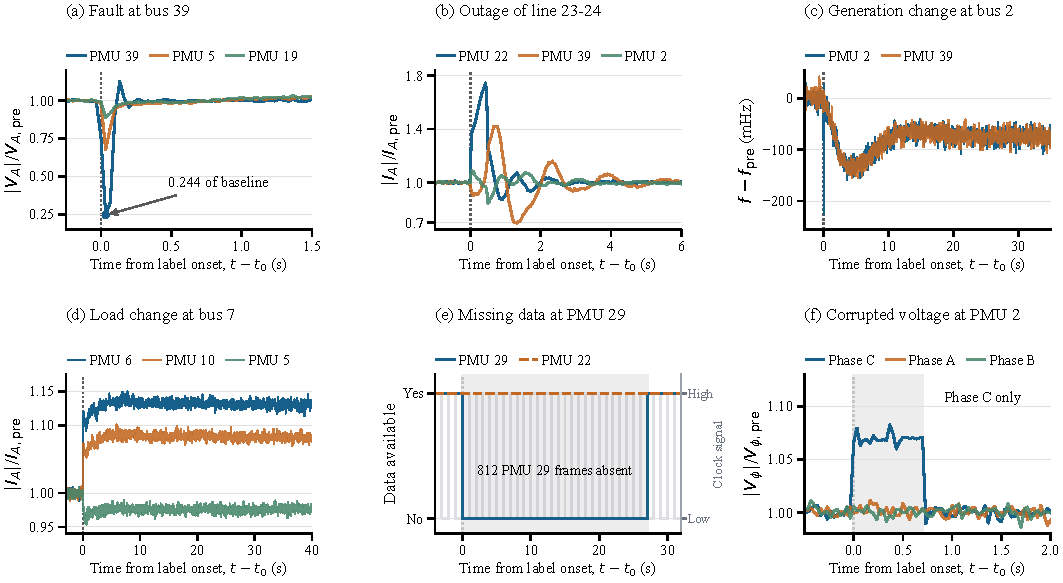
\includegraphics[width=\textwidth]{figures/generated/event_signatures.pdf}
\caption{Representative measured signatures from the RAW0001 reference simulation. Physical events alter voltage, current, or frequency through the network; integrity events alter availability or channel consistency. In panel (e), the gray reference clock advances while PMU~29 packets are absent. Curves are unsmoothed, and each panel uses the time scale needed to show its physical response.}
\label{fig:event-signatures}
\end{figure*}

All intervals and tests use the experiment's independent unit: a complete trajectory, event parent, or rebuilt plant. Generated tables and figures read only the hashed frozen snapshot. Sample-level PMU frames are never promoted to independent replicates.

\subsection{Status of the Single-Event Pilot}
The multi-family pilot in Section~\ref{sec:single-event-route} has a different provenance tier. Two author-supplied technical dossiers dated September~24, 2026 summarize its campaign packages, but the underlying solver logs, frozen manifests, and final-survivor archive are not present in this repository. Its four development cases, four blind mini-holdout cases, and four quiet controls are independent \emph{cases}, not a population performance sample; no interval or false-alarms-per-hour estimate is computed from them. We report this line as an exploratory engineering audit in Section~\ref{sec:pilot-results} and Supplementary Appendix~H. None of its numerical values is pooled with RQ1--RQ4 or promoted to the abstract's primary evidence.

\section{State Evidence From Recovery to Model Failure}
\label{sec:nominal-results}

\subsection{RQ1 Measurement Conditioning Recovers the Target}

The estimator sequence reveals where the nominal accuracy comes from. Conditioning the equilibrium on the current PMU frame (B1) reduces hidden-voltage error by more than one order of magnitude. Adding causal propagation (B2) improves most trajectories, but by a much smaller amount. Thus the network-constrained measurement map supplies the main gain; temporal propagation refines it.

\begin{table*}[t]
\caption{Nominal reconstruction on 100 frozen nonlinear TEST trajectories. Metrics use the 31 unobserved buses only; TVE is reported in percent and intervals bootstrap independent trajectories.}
\label{tab:nominal-results}
\centering
\footnotesize
\begin{tabular}{lccccc}
\toprule
Method & Complex RMSE & $|V|$ RMSE & Angle RMSE ($^\circ$) & Mean TVE (\%) & 95\% TVE interval (\%) \\
\midrule
B0 equilibrium & 3.486e-03 & 2.496e-05 & 0.19497 & 0.340200 & [0.293231, 0.387428] \\
B1 snapshot WLS & 1.529e-04 & 5.091e-05 & 0.00821 & 0.009904 & [0.008342, 0.011514] \\
B2 causal Kalman & 1.338e-04 & 4.235e-05 & 0.00722 & 0.009634 & [0.008006, 0.011302] \\
\bottomrule
\end{tabular}
\end{table*}


Figure~\ref{fig:nominal-reconstruction}(a) shows the scale change directly, and panel (c) uses paired trajectory differences rather than overlapping marginal intervals. The comparison is deliberately internal: B0, B1, and B2 share the same local physical model. It does not claim superiority over every learned or nonlinear estimator.

\begin{figure*}[t]
\centering
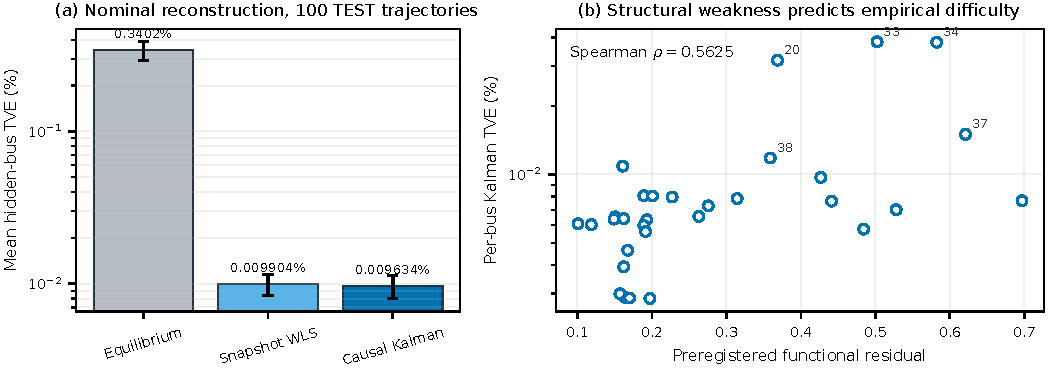
\includegraphics[width=\textwidth]{figures/generated/nominal_reconstruction.pdf}
\caption{Where nominal state-reconstruction accuracy comes from. (a) PMU conditioning produces the dominant reduction in trajectory-level hidden-voltage error. (b) The preregistered structural residual predicts some, but not all, difficult buses. (c) Paired B2-minus-B1 differences isolate the smaller contribution of causal propagation.}
\label{fig:nominal-reconstruction}
\end{figure*}

The structural residual in Fig.~\ref{fig:nominal-reconstruction}(b) correlates with bus-level B2 error, but the relationship is incomplete. The buses share trajectories and network coupling, and the residual comes from the threshold-sensitive projector discussed in Section~\ref{sec:functional-observability}. It is therefore a difficulty indicator, not an observability certificate.

Two negative checks sharpen this result. The fixed-lag smoother does not improve the nonlinear TEST trajectories, even though a correctly specified linear-Gaussian smoother cannot increase expected squared error. Innovation autocorrelation identifies the missing premise: the local model treats deterministic governor and load excitation as white process noise. Marginal temperature scaling repairs coverage under nominal operation but does not whiten those innovations. More data cannot compensate for the wrong temporal model.

\subsection{RQ2 Physical Shift Exposes the Model Boundary}

The mismatch campaign asks whether nominal accuracy survives a changed plant. It does not fail uniformly. Network-parameter changes and operating-point shifts dominate the state error, while the tested machine, governor, AVR, and load-model perturbations remain close to the nominal level over the short excitation [Fig.~\ref{fig:physical-mismatch}(a)]. Those near-null responses show that the experiment did not expose the corresponding parameters; they are not evidence of general robustness.

\begin{figure*}[t]
\centering
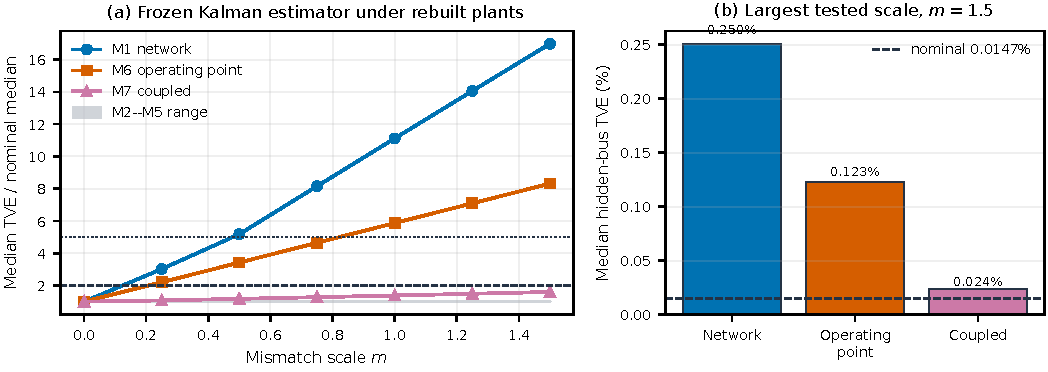
\includegraphics[width=\textwidth]{figures/generated/physical_mismatch.pdf}
\caption{How the frozen state estimator fails under physical mismatch. (a) Network and operating-point changes dominate the hidden-voltage error. (b) A covariance correction fitted under nominal operation loses coverage after physical shift. (c) Observed innovations often flag unacceptable hidden error but do not identify its physical cause. Each family-scale cell contains 20 rebuilt plants.}
\label{fig:physical-mismatch}
\end{figure*}

This pattern suggests a mechanism. A stale equilibrium moves the center of both the measured and hidden voltage fields. The offset-only ablation estimates that movement from measured buses but ignores AC balance, and it closes almost none of the oracle gap. The constrained recentering in \eqref{eq:e06h-map} instead rebuilds a physically admissible center. Across all three held-out operating shifts, it removes nearly all of the point-error gap [Fig.~\ref{fig:adequacy-adaptation}(a)--(b)].

\begin{figure*}[t]
\centering
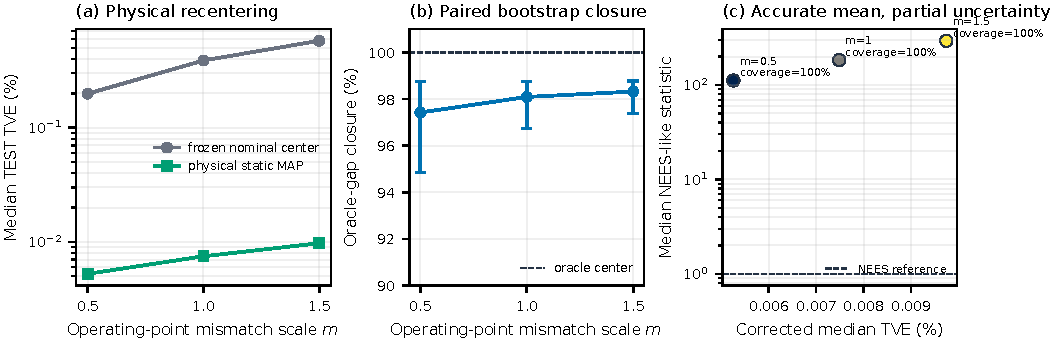
\includegraphics[width=\textwidth]{figures/generated/adequacy_adaptation.pdf}
\caption{Physical recentering separates point recovery from uncertainty. (a) Enforcing the AC map sharply reduces hidden-voltage error under operating-point shift. (b) The paired oracle-gap closure is consistent across held-out cases. (c) The joint NEES-like diagnostic remains too large even when marginal intervals cover, so the point estimate is supported but its joint covariance is not.}
\label{fig:adequacy-adaptation}
\end{figure*}

\begin{table*}[t]
\caption{Corrected physical static recentering on 60 held-out M6 operating-point cases. Gap-closure intervals bootstrap the 20 independent TEST cases at each scale. Rank and nullity refer to the 43-dimensional nuisance basis; runtime is per solve.}
\label{tab:e06h-results}
\centering
\footnotesize
\begin{tabular}{ccccccccc}
\toprule
$m$ & $n$ & Frozen TVE (\%) & Corrected TVE (\%) & Gap closure [95\% CI] (\%) & Rank & Nullity & Median NEES & Runtime (ms) \\
\midrule
0.5 & 20 & 0.19885 & 0.00525 & 97.4 [94.9, 98.8] & 25/43 & 18 & 111.6 & 57.6 \\
1.0 & 20 & 0.38834 & 0.00749 & 98.1 [96.7, 98.8] & 25/43 & 18 & 183.3 & 61.1 \\
1.5 & 20 & 0.57795 & 0.00974 & 98.3 [97.4, 98.8] & 25/43 & 18 & 294.2 & 69.2 \\
\bottomrule
\end{tabular}
\end{table*}


The recovery does not identify every operating-point coordinate. The nuisance information is rank deficient, yet the requested voltage field changes little along much of that nullspace. This is the empirical counterpart of Proposition~\ref{prop:functional-reconstruction}: a target can be recoverable even when the full latent vector is not. The remaining limitation is uncertainty. Marginal intervals cover, but the joint NEES-like statistic is severely under-dispersed, and the independent constrained solver converges on only part of its small diagnostic subset. The evidence supports point reconstruction for the tested operating shifts, not joint parameter recovery or sequential adaptation.

\section{Event Evidence From Detection to Source Ambiguity}
\label{sec:results}

\subsection{RQ3 Cardinality Resolves Before Exact Support}

The prospective test opens the full 137-hypothesis bank only after the physical dictionary, covariance, priors, onset, and numerical integration are frozen. Every source pair competes in one normalized posterior. The resulting pattern is monotone with event strength, but the two decisions do not improve at the same rate (Table~\ref{tab:global137-results}). Finite pairs are recovered exactly, whereas weak--weak Top-1 remains \GlobalWeakTopOne{}. Weak sources are therefore the decisive regime, not a small perturbation around an otherwise uniform accuracy claim.

\begin{table*}[t]
\caption{Fresh prospective 137-hypothesis confirmation. The bank contains $H_0$, 16 single-source hypotheses, and all 120 two-source supports. Repeated noise realizations are decisions, not independent physical trajectories. Top-$k$ is exact support recovery and is undefined for $H_0$ and single-source rows in this exported support table.}
\label{tab:global137-results}
\centering
\footnotesize
\begin{tabular}{lrrrrrr}
\toprule
Regime & Physical trajectories & Decisions & Cardinality (\%) & Top-1 (\%) & Top-3 (\%) & Mean $p(K=2)$ \\
\midrule
No event & --- & 100 & 100.0 & --- & --- & 0.000 \\
Single source & 128 & 384 & 93.8 & --- & --- & 0.051 \\
Weak--weak pair & 1920 & 5760 & 37.4 & 24.4 & 59.8 & 0.427 \\
Weak--strong pair & 480 & 1440 & 77.6 & 66.2 & 95.8 & 0.808 \\
Moderate pair & 480 & 1440 & 99.7 & 98.8 & 100.0 & 0.996 \\
Finite pair & 480 & 1440 & 100.0 & 100.0 & 100.0 & 1.000 \\
\bottomrule
\end{tabular}
\end{table*}


Figure~\ref{fig:multi-event-evidence} follows the inference failure in the same order as the method. Panel (a) establishes the strength-dependent recovery boundary. Panel (b) then shows that evidence for $K=2$ grows while exact pair recovery remains nearly flat. The model has detected multiplicity before it has localized the support. Reporting only event detection would hide this failure.

\begin{figure*}[t]
\centering
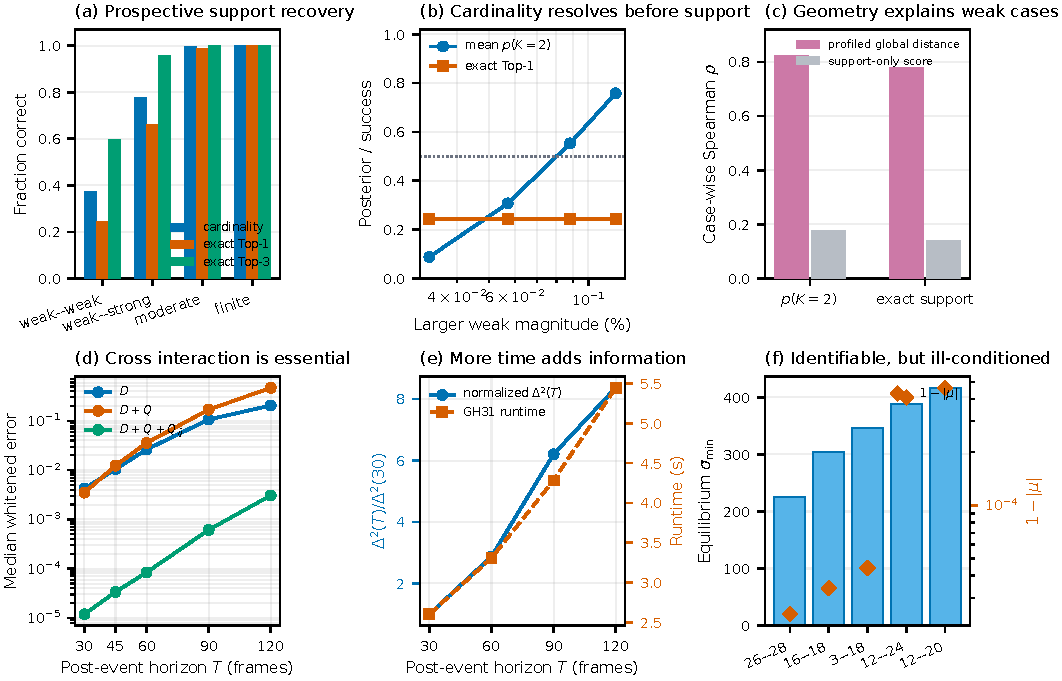
\includegraphics[width=\textwidth]{figures/generated/multi_event_evidence.pdf}
\caption{Why simultaneous-source recovery fails in the weak regime. Prospective results first separate cardinality from exact support (a--b). Retrospective geometry then links weak-case errors to profiled response distance (c). The longer-horizon diagnostic shows that the pairwise interaction is needed (d), information accumulates with time (e), and distinct equilibrium signatures can remain nearly collinear (f). Panels (c)--(f) explain the result but do not replace a prospective recovery test.}
\label{fig:multi-event-evidence}
\end{figure*}

Event presence is easier than source recovery. The frozen detector separates most event and no-event records, but its no-event exposure is too short for an operational false-alarm claim. Per-bus inclusion probabilities also rank useful candidates, yet their missed-source rate remains too high to repair weak exact-support decisions. Supplementary Appendix~G reports these secondary metrics and denominators.

\subsection{Profiled Geometry Explains the Weak Cases}

The retrospective audit asks why the weak bank fails. A support-only score compares candidate signatures while holding the rest of the explanation fixed. The profiled distance instead allows the competing support to choose its best amplitude and thereby measures the actual overlap between response manifolds. The latter tracks exact weak-case recovery far more closely [Fig.~\ref{fig:multi-event-evidence}(c)].

This result changes the interpretation of the weak regime. Every tested direction is first-order resolvable, so a curvature-dominated $a^{-4}$ delay law is not the observed mechanism. The errors arise because several finite-horizon candidate responses lie close after amplitude profiling. Detectability and source identity therefore require different geometric quantities.

The first-order theory separates two reasons for that proximity. A source may have
little response outside the nuisance span, or it may remain visible but nearly
collinear with another source after nuisance removal. Shared-source competitors
make the second mechanism especially severe because their common component
cancels before the exclusive source is compared. The frozen audit uses the full
nonlinear profiled distance and supports this explanation retrospectively; it does
not yet validate the analytic small-amplitude coefficient in
\eqref{eq:support-to-support-margin}.

The 120-frame diagnostic adds a second piece of the explanation. Extending the window increases the separation proxy by more than eightfold, and no candidate pair is exactly degenerate in the frozen equilibrium model. Yet the hardest signatures remain almost collinear [Fig.~\ref{fig:multi-event-evidence}(e)--(f)]. More time adds information without guaranteeing a well-conditioned decision.

The physical-manifold check also shows why the nonlinear interaction in \eqref{eq:load-multi-source-mean} cannot be dropped. Adding only single-source curvature does not improve the simultaneous response; adding $\bm Q_{ij}$ reduces the median whitened error by roughly two orders of magnitude [Fig.~\ref{fig:multi-event-evidence}(d)]. This check covers 32 nominal-operating-point paths. It validates the representation locally, not population recovery at 120 frames or robustness to operating shift.

\subsection{RQ4 Source Labels Do Not Generalize to New Assets}

The supervised hierarchy provides a useful contrast. On the ordinary split it detects events and ranks known sources well, confirming that multiscale dynamics, adaptive residuals, and PMU contrasts carry event information. That result answers interpolation at represented assets.

The source-holdout result answers a different question. With the physical asset removed from all source-labeled fitting and the true event family supplied, only \HeldSourceCorrect{} of \HeldSourceDecisions{} decisions are exact. The failure remains after detection and family confusion have been removed. The location heads and asset descriptors therefore memorize source-specific associations that do not transfer to an unseen physical source.

The physical load bank avoids that shortcut by generating a response for every candidate support. Its success is narrower in another direction: it covers only load interventions under fixed topology, known onset, matched operation, and synthetic noise. Together, the two experiments motivate the next model rather than a claim of general superiority: learned residuals should correct a physical candidate likelihood and must be tested on event parents and source assets excluded from training.

\subsection{Exploratory Multi-Family Pilot: Search Survives, Selection Does Not}
\label{sec:pilot-results}

The single-event pilot tests a different bottleneck from the load-support bank: can the true physical explanation remain in a tractable four-family shortlist when onset and severity are fitted? The author-supplied campaign summaries report that a development-selected, frozen screening and racing policy retained the true candidate in all four blind mini-holdout cases (one fault, load change, generator change, and line outage). The generator case reached the six-survivor cutoff with no spare place. Four quiet windows provided only a pilot check of proposal scores; they cannot establish operational false-alarm control. The solver diagnostics also report full-block/Schur agreement on 30 synthetic systems and fault-resistance estimates of 0.02006--0.02133 from four initializations around a synthetic truth of 0.021. These checks establish numerical behavior of components on the reported cases, not a validated source-localization rate.

The same dossiers report a negative strict-final outcome: none of the four truth candidates won the final comparison. That 0/4 is currently a terminal-reported result without its matching final-survivor archive in the repository. Its mechanisms must remain distinct. Fault and line truth/competitor fits did not all reach strict convergence, so their ranking is numerically unresolved. In the load and generator cases, converged neighboring same-family candidates reportedly received better final scores. That pattern motivates an oracle sequence for event-operator parity, pre-event state, onset and duration, severity, noise, and counterfactual PMU coverage. It does not yet prove an intrinsic identifiability limit. The pilot thus supports continued work on the joint numerical route but supplies no positive multi-family end-to-end claim. Supplementary Appendix~H gives the case ledger, reported diagnostics, and the exact artifact checks needed to turn this audit into primary evidence.

\subsection{Unknown-Onset Continuous Evidence: Scope and Failure Modes}
\label{sec:continuous-evidence}

The continuous component is evaluated separately from the prospective batch bank. Two completed development campaigns, H03 and H04, each contain three 80-s event parents with six successive load/line interventions and one normal parent. The same schedules are paired across nominal, in-bank R/X, and out-of-bank mixed R/X conditions. Thus each campaign contains 18 unique interventions and 54 paired event realizations. All use F01 operation, one instrumental-noise level, eight fixed PMUs, and the known nine-load/nine-line catalog. Neither campaign demonstrates unseen-source generalization. They are now development evidence and cannot be reused as a new blind confirmation.

In H03, R11 obtains \ContPriorTimely{}/54 correct family/source decisions before physical restoration, with \ContPriorExtras{} unmatched alarms. Table~\ref{tab:continuous-h04} reports the subsequent H04 outcomes. R11 retains \ContMixTimely{}/\ContMixTotal{} timely decisions, whereas its nominal ablation retains \ContNomTimely{}/\ContNomTotal{}. The mixture has fewer extras (\ContMixExtras{} versus \ContNomExtras{}), but loses one timely attribution. Parameter uncertainty therefore yields a trade-off, not uniform dominance. Under out-of-bank R/X, timely BUS31 attribution is \ContMixBusTimely{}/3 for the mixture and \ContNomBusTimely{}/3 for the nominal ablation. Eventual correct attribution would conceal that delay.

\begin{table}[t]
\centering\small
\caption{Executed continuous-stream development evidence (H04). Timely means correct family/source emitted before physical restoration; extras are unmatched alarms. OUT denotes out-of-bank R/X; F1 is report-level detection F1. These are paired realizations of 18 events from three event parents, not 54 independent events.}
\label{tab:continuous-h04}
\resizebox{\columnwidth}{!}{%
\begin{tabular}{lrrrr}
\toprule
Method & Timely & Extras & OUT timely & OUT F1\\
\midrule
R11 mixture & 53/54 & 4 & 17/18 & 0.818\\
R11 nominal & 54/54 & 7 & 18/18 & 0.828\\
Admission ablation & 52/54 & 0 & 16/18 & 0.854\\
ExtraTrees reference & 27/54 & 3 & 9/18 & 0.619\\
ExtraTrees short & 27/54 & 3 & 9/18 & 0.626\\
\bottomrule
\end{tabular}}
\end{table}


\begin{figure*}[t]
\centering
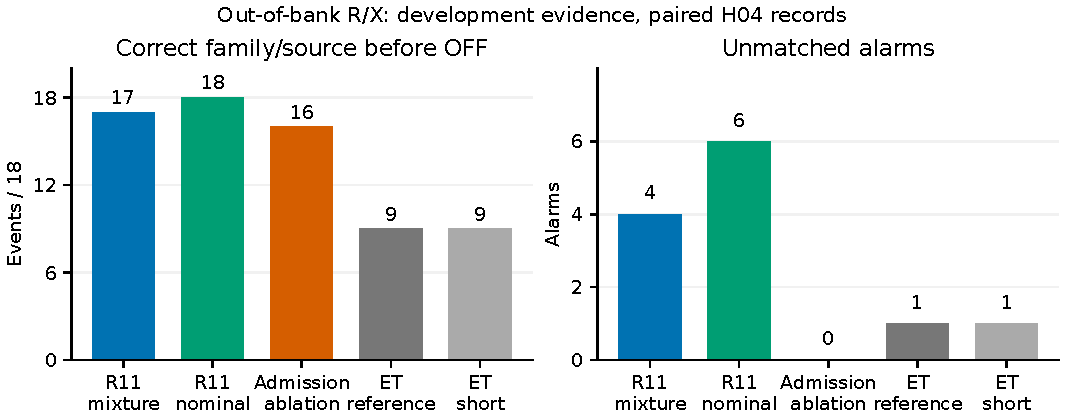
\includegraphics[width=0.92\textwidth]{figures/generated/continuous_tradeoff.pdf}
\caption{Failure trade-off under out-of-bank network error in H04. An additional causal-admission ablation eliminates unmatched alarms but rejects a real BUS16 intervention; the nominal R11 retains every timely event but has more extra alarms. These paired development results do not establish a universally superior variant.}
\label{fig:continuous-tradeoff}
\end{figure*}

An additional admission ablation retains \ContAdmissionTimely{}/\ContAdmissionTotal{} timely decisions with \ContAdmissionExtras{} extras. Its zero-extra result is insufficient for promotion: it rejects a true BUS16 load intervention whose retrospective onset lacks the required early witness. The change reduces public alarms while leaving the inherited physical states and hypothesis masses unchanged. We retain it as negative evidence rather than silently replacing R11. Both R11 references are now frozen; no bus-specific correction follows these observations.

The two frozen ExtraTrees adaptations obtain \ContETTimely{}/\ContMixTotal{} timely decisions here. This is an identical-stream causal comparison under the restricted load/line contract, not a recomputation of the hackathon leaderboard or an assertion about all event classes. Report-level F1 and event-level timely attribution measure different targets and are shown separately. The short normal exposure and three event parents cannot support a precise operational false-alarm rate or generalization confidence interval.

The published physical comparator passes equation-level tests for the reduced network, partial-observation marginalization, Gaussian log-likelihood, suffix-max recursion, angle wrapping, and stopping localization. On independently generated three-bus sequences under its own Gaussian law, \ChenMatchedCorrect{}/\ChenMatchedTotal{} post-change trials stop after onset at the correct line; \ChenMatchedEarly{} trial stops before the change. No alarm occurs over \ChenNormalExposure{} normal increments, with every normal sequence right-censored at its observation horizon. This checks an implementation under matched assumptions, not the numerical results of the original article. On three previously opened F01 normal records, the adapter alarms in all three; colored noise and frame dynamics violate its assumed law. We preserve that mismatch result and make no general superiority claim from it.

The confirmatory C01 configuration is sealed before its new draw. It specifies independent physical parents, longer normal records, paired R/X conditions, two instrumental-noise scales, persistent-line eligibility for the published comparator, and paired parent-cluster intervals. Both R11 references and both ExtraTrees artifacts remain fixed. Solver rejects, inference failures, late decisions, and right-censoring remain in the ledger. C01 has not been executed; it contributes no performance number to this manuscript. Source-disjoint inference, changing PMUs, faults, generation interventions, and the complete joint estimator remain outside this confirmatory contract.

\section{Discussion and Limitations}
\label{sec:discussion}

The experiments support one central distinction: recovering a requested state function is not the same as identifying the intervention that produced it. The state estimator can reconstruct hidden voltages because many unobservable state directions have little effect on that target. Source inference is stricter. It must separate every admissible candidate after amplitude and other nuisance directions are allowed to adjust.

The state results make this distinction concrete. Instantaneous PMU conditioning supplies most of the nominal improvement, while causal propagation adds a smaller correction. When the equilibrium becomes stale, an unconstrained offset does not solve the problem; rebuilding an AC-feasible center does. The resulting point estimate is accurate even though the operating-point coordinates remain non-unique. Its joint covariance is still unreliable. Target recovery and parameter recovery must therefore be evaluated separately.

An archived ANDES calibration checkpoint makes the parameter distinction more
concrete. Individual screening retained 10 of 18 directions, but their joint
condition number was 722.9. Rank-revealing selection reduced the set to eight
directions with condition number 7.83, and a final $6.15\sigma$ displacement
gate left seven in the released local posterior. The rejected directions did
not share one explanation: six were information-poor, two violated the local
curvature gate, two added little first-order direction, and one left the local
model domain. Supplementary Appendix~D traces these counts to the frozen gate
ledger. Because the checkpoint lacks the required higher derivatives, it does
not establish which rejected directions are curvature-resolved or structurally
redundant.

The event results expose a parallel hierarchy. Weak simultaneous events often provide enough evidence for two active sources before they identify the pair. Profiled manifold distance explains this behavior because it measures what remains after a competing support chooses its best amplitude. Longer observation increases that distance, but nearly collinear signatures still amplify noise. A positive structural margin is therefore a uniqueness statement, not a reliability guarantee. This information--delay trade-off has a measurement-level analogue: our previous benchmark showed disturbance-dependent trade-offs among transient error, settling behavior, observation characteristics, and computational cost across dynamic frequency estimators \cite{Mayorga2026FrequencyBenchmark}. In the present problem, the corresponding trade-off occurs at the inference level: longer PMU histories can increase physical source separation while delaying the localization decision.

The supervised baseline adds a warning about learning. Engineered temporal and spatial features work when the source appears in training. Under complete source holdout, the same representation loses source identity even when the event family is supplied. A learned correction should therefore operate on candidate residuals, not on asset labels alone, and its value must be measured against the physics-only likelihood on the same event parents.

The evidence remains bounded in four ways. First, the state and event paths are evaluated separately rather than as one fitted posterior. Second, the Bayesian support result covers one event family, fixed topology, known onset, fixed PMUs, and matched operation. Third, the 120-frame study is diagnostic and lacks independent operating-point validation. Fourth, the normal exposure is too short to establish false alarms per hour, and no field or cross-simulator validation is claimed.

The separate continuous component supplies unknown-onset load/line evidence under a fixed catalog, but leaves those broader gaps open. Its frozen observation intercept corrects the measured residual center; it does not contradict the hidden-state study's finding that an arbitrary offset cannot replace AC-feasible recentering. Likewise, its finite network mixture does not identify true R/X or establish calibrated probabilities. The nominal component's better timely attribution and worse alarm burden make both references necessary.

The next decision is a finite confirmatory comparison, not another bus-specific repair. The sealed C01 protocol compares those fixed references and the frozen ExtraTrees adaptations on continuous records, and compares the published physical detector only on persistent-line and normal records. It retains failed and censored cases. That campaign can validate the stated restricted causal contract; it cannot establish source-disjoint transfer, a learned-discrepancy benefit, changing-PMU robustness, or the complete joint estimator. Those claims remain blocked rather than inferred from improved development scores.

\section{Conclusion}
\label{sec:conclusion}

Sparse PMUs impose different information limits on state reconstruction and event-source inference. The requested hidden-voltage function can be estimated accurately even when the full local state is not observable. Event support requires a stronger condition: candidate responses must remain separated after amplitude and nuisance directions are profiled.

The experiments follow that logic. Eight PMUs reconstruct the 31 unmeasured bus voltages with \BTwoTVE{} mean relative error under the matched model, and physical recentering repairs most of the tested operating-point shift. In the prospective load bank, finite two-source supports are recovered exactly, whereas weak-pair Top-1 remains \GlobalWeakTopOne{}. The gap is explained by finite-horizon response overlap and near-collinearity, not by event absence alone.

The present evidence supports matched-model state reconstruction and simultaneous load-source inference as separate components. A separate causal load/line component obtains \ContMixTimely{}/\ContMixTotal{} timely decisions with \ContMixExtras{} unmatched alarms in development streams, while its nominal ablation retains one more timely event at a higher alarm burden. That trade-off and the negative admission ablation are part of the result. R11 and its nominal ablation are frozen for a preregistered comparison with ExtraTrees and an implemented published line-outage detector. No confirmatory outcome is claimed before execution. The complete multi-family state/event/integrity posterior, source holdout, changing sensing, and field transfer remain open.

\section*{Supplementary Material}

The companion supplement contains the paper-by-paper literature matrix, electrical and PMU conventions, proofs, complete estimator equations, frozen experimental contracts, and secondary result tables. These details preserve reproducibility without interrupting the main scientific argument.


% Acknowledgments and author biographies are intentionally omitted until author-provided.
\bibliographystyle{IEEEtran}
\bibliography{references}

\EOD
\clearpage
\IfFileExists{\PSevenSupplementPDF}{%
  \includepdf[
    pages=-,
    fitpaper=true,
    pagecommand={\thispagestyle{empty}},
    addtotoc={1,section,1,{Supplementary Material},supplementary-material}
  ]{\PSevenSupplementPDF}%
}{%
  \PackageError{P07}{Supplementary PDF not found}{Run scripts/build_manuscript_bundle.ps1 before compiling main.tex.}%
}
\end{document}
